\documentclass{report}
%Math Stuff
\usepackage{amsmath}
\usepackage{enumitem}
\usepackage{mathtools}

%General Formating
\usepackage[letterpaper, portrait, margin=1in]{geometry}
\usepackage{fancyhdr}
\pagestyle{fancy}

%Bibliography
\usepackage[toc,page]{appendix}
\usepackage{hyperref}

%Figures
\usepackage{graphicx}
\graphicspath{ {figures/} }
\usepackage{tikz}
\usepackage{pgfmath}
\usepackage{framed}
\usepackage{csvsimple}

%Header
\lhead{Schulman}
\rhead{Page \thepage}

%Title
\title{Food Networks \\~\\ \normalsize A Thesis Presented to the Faculty of the Economics Department of Cornell University in Partial Fulfillment of the Requirements for the Degree of Bachelor of Arts in Economics with Honors} 
\author{Eric Schulman}
\date{May 2017}

\begin{document}

\maketitle

\pagebreak

\begin{abstract}
For my thesis, I ask how produce prices relate to the structure of the network of farms, intermediate buyers, and stores. To answer this question, I estimate the relative cost of transporting grapes, cabbage, onions, and cherries for each census tract in New York State. My estimates come from an optimization problem specified using publicly available sattelite data regarding crop cover and New York's records on food vendor permits. I solve the problem using linear programming software packages. All of the code to used to complete this project is publicly available on GitHub at \url{http://github.com/erichschulman/ag_networks}.
\end{abstract}

\pagebreak

\renewcommand{\abstractname}{Acknowledgements}
\begin{abstract}
I wanted to thank Professor Patacchini for advising the project, Professor Besharov for running the honors program. I should also thank Professor Tardos for helping me to understand the algorithms involved with this project. I also want to thank Professor Easley and Professor Caunedo for their help. 
\end{abstract}

\tableofcontents

\chapter{Background}

\section{Related Work}

\subsection{Demographics, Policy and Nutrition}

Researchers have studied the statistical relationship between transfer programs, demographics and nutritional outcomes for a long time. Calculating these statistical relationships is straightforward for the US because the Census Bureau publishes a monthly current population survey monthly and nutrition supplement. 

This literature finds reducing costs and increasing availability of nutritional foods improves health outcomes. One study evaluated the Farmers' Market Nutrition Program, a national program intended to increase consumption of fresh fruits and vegetables by providing coupons and information. Researchers found subsidizing nutritionally rich food with coupons leads to increased consumption when complemented with information \cite{Just}. The literature also found nutritional outcomes are related to systemic factors. For example, researchers analyzed nutritional outcomes in Oregon between 1999 and 2001, when Oregon had the highest average rate of hunger in the nation. The study found county-level factors like residential location and housing costs were most related to food insecurity \cite{Bernell}. 


\subsection{Spatial Data and Nutrition}

Researchers realized state-level data has its limitations limitations. To understand systemic nutritional patterns, researchers began describing food supply in detail using spatial coordinates and mapping software.  One study conducted among grocery stores across inner cities and suburbs within the Minneapolis and St. Paul metropolitan concluded the urban poor pay marginally more for food because supermarket chains don't open in inner cities \cite{Chung}. Researchers began applying the label "food deserts" to inner cities. With more data becoming available online, researchers continue describing food supply in more detail to understand systemic food insecurity. In one project, researchers leveraged Google Maps, and local online news to build a graphical representation of food availability in Bogota, Columbia \cite{Hwang}. Another study used online directories of grocery stores to index neighborhoods' vulnerability to food insecurity in the twin cities area \cite{Larson}.
 
\subsection{Optimization Problem and Food}

Food allocation is closely related with nutrition and often studied using a transportation problem. Transportation problems are an optimization problem designed to find the cheapest possible way of sending a certain amount of supply through a network. A typical application of this problem involves finding the best delivery route from a factory to a warehouse where the road network has some capacity and cost associated. Solving the problem involves finding a vector with an economic interpretation of optimal prices from a social planning perspective. It can be solved efficiently using the network simplex algorithm and linear programming software packages \cite{Cook}. Researchers have often applied transportation problems to food allocation. One paper studies maize allocation in South Africa where rails carry maize from supply and demand points, scattered throughout the country. Researchers minimize the total rail cost, as is standard, but add a secondary objective of distributing costs fairly among all users \cite{Stewart}.

\section{Optimal Transportation}

I've decided to devote a section of my thesis explaining the nature of the optimization problem I specify and solve. My chosen application for the transportation problem is novel, but the problem its self is not. It's actually taught in most undergraduate optimization courses\cite{Cook}. Since I recognize that this is a different direction than other economics thesis projects from the past, I want to make sure it's clear what I've done and the tools that I used to do it.

\subsection{Problem Description}

The optimization problem plan to specify and solve is called a transportation problem. It actually has a few names. It's usually called minimum-cost flow. This is because the it tries to maximize the amount of flow (in my case units of goods flowing through a network) at the minimum cost. It's essentially a more general version of a matching market. There are suppliers and demand-ers connected in a network. Like a matching market, the goal is to match supply with demand. The catch is that edges in this problem are not all equal. Certain edges are more expensive than others. The difference betweeen this and a normal matching market is that this problem tries to find the cheapest possible way to match supply with demand. The problem inputs are list of suppliers and demand-ers with capacities and edges with costs. It tells you how much of each good each supplier should send to each demand-er.

\subsection{Solving the Problem}

Finding the minimum cost of sending goods through the network works a lot like finding the optimal matching for a matching market. You can start by maximizing the amount of goods you've sent through the network without worrying about cost. This works exactly like a normal matching market. You can use the augmenting path to do this. After finding the maximum amount of goods flowing through the network, the algorithm tries to find the optimal cost. You do so by finding a reduced cost path. This works exactly like an augmenting path in a matching market. You start at a supply node and trace a path alternating between supply and demand until you reach your original node. If you can trace back to your initial node then you've reduced the cost. You repeat this process until you've exhausted all of the reduced cost cycles.


\subsection{Worked out Example}

To get a better sense of the problem and how to solve it, I've worked out an example of a transportation problem with a network of 5 nodes. You can see in Figures \ref{fig:example1} through \ref{fig:example6} how the algorithm works.

\begin{figure}
\centering
\begin{framed}
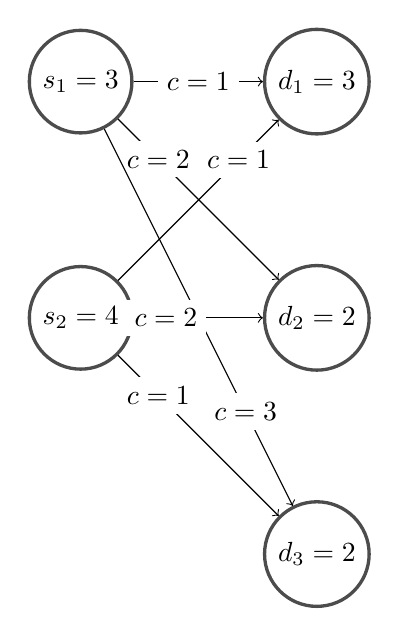
\begin{tikzpicture}[
node/.style={circle, draw=black!70, fill=white!5, very thick, minimum size=9mm}
]
%Nodes
\node[node]      (s1)                                        {$s_1= 3$};
\node[node]      (s2)     [below of =s1, yshift= -2cm]       {$s_2 = 4$};
\node[node]      (d1)     [right of =s1 , xshift= 2cm]       {$d_1 = 3$};
\node[node]      (d2)     [below of = d1, yshift= -2cm]       {$d_2 = 2$};
\node[node]      (d3)     [below of = d2, yshift= -2cm]      {$d_3 = 2$};
%Lines
\draw[->] (s1) -- (d1) node [midway, fill=white] {$c= 1$};
\draw[->] (s1) -- (d2) node [near start, fill=white] {$c = 2$};
\draw[->] (s1) -- (d3) node [near end, fill=white] {$c = 3$};
\draw[->] (s2) -- (d1) node [near end, fill=white] {$c = 1$};
\draw[->] (s2) -- (d2) node [near start, fill=white] {$c = 2$};
\draw[->] (s2) -- (d3) node [near start, fill=white] {$c = 1$};
\end{tikzpicture}
\caption{This picture represents the network for which we will be finding minimum cost flow. The supply and demand nodes are labeled with their corresponding capacities.  The edges between each supply and demand node are labled according to their cost. To make the problem easier, you can assume all edges have unlimited capacity meaning suppliers can send as much goods as they want over them.}
\label{fig:example1}
\end{framed}
\end{figure}

\begin{figure}
\centering
\begin{framed}
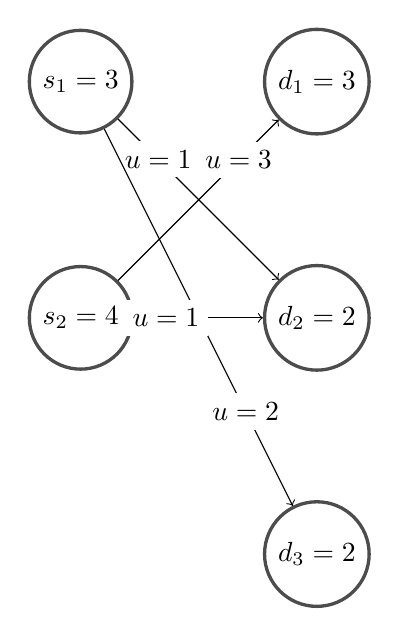
\begin{tikzpicture}[
node/.style={circle, draw=black!70, fill=white!5, very thick, minimum size=9mm}
]
%Nodes
\node[node]      (s1)                                        {$s_1= 3$};
\node[node]      (s2)     [below of =s1, yshift= -2cm]       {$s_2 = 4$};
\node[node]      (d1)     [right of =s1 , xshift= 2cm]       {$d_1 = 3$};
\node[node]      (d2)     [below of = d1, yshift= -2cm]       {$d_2 = 2$};
\node[node]      (d3)     [below of = d2, yshift= -2cm]      {$d_3 = 2$};
%Lines
\draw[->] (s1) -- (d2) node [near start, fill=white] {$u = 1$};
\draw[->] (s1) -- (d3) node [near end, fill=white] {$u = 2$};
\draw[->] (s2) -- (d1) node [near end, fill=white] {$u = 3$};
\draw[->] (s2) -- (d2) node [near start, fill=white] {$u = 1$};
\end{tikzpicture}
\caption{The algorithm starts by matching the capacities on the supply nodes with the capacities on the demand nodes. This is trivial because there are no edge capacities and every node is connected.}
\label{fig:example2}
\end{framed}
\end{figure}

\begin{figure}
\centering
\begin{framed}
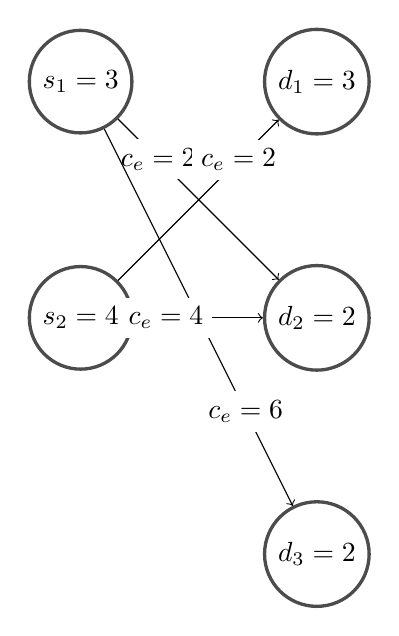
\begin{tikzpicture}[
node/.style={circle, draw=black!70, fill=white!5, very thick, minimum size=9mm}
]
%Nodes
\node[node]      (s1)                                        {$s_1= 3$};
\node[node]      (s2)     [below of =s1, yshift= -2cm]       {$s_2 = 4$};
\node[node]      (d1)     [right of =s1 , xshift= 2cm]       {$d_1 = 3$};
\node[node]      (d2)     [below of = d1, yshift= -2cm]       {$d_2 = 2$};
\node[node]      (d3)     [below of = d2, yshift= -2cm]      {$d_3 = 2$};
%Lines
\draw[->] (s1) -- (d2) node [near start, fill=white] {$c_e = 2$};
\draw[->] (s1) -- (d3) node [near end, fill=white] {$c_e = 6$};
\draw[->] (s2) -- (d1) node [near end, fill=white] {$c_e = 2$};
\draw[->] (s2) -- (d2) node [near start, fill=white] {$c_e = 4$};
\end{tikzpicture}
\caption{This solution is not optimal in terms of cost (yet). I've labled each edge in this figure with the cost each edge has incurred. It works out to 14. The edge costs are just the amount of flow on each edge times its cost.}
\label{fig:example3}
\end{framed}
\end{figure}

\begin{figure}
\centering
\begin{framed}
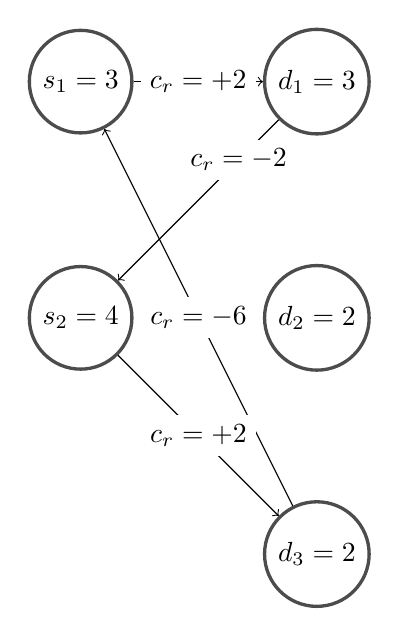
\begin{tikzpicture}[
node/.style={circle, draw=black!70, fill=white!5, very thick, minimum size=9mm}
]
%Nodes
\node[node]      (s1)                                        {$s_1= 3$};
\node[node]      (s2)     [below of =s1, yshift= -2cm]       {$s_2 = 4$};
\node[node]      (d1)     [right of =s1 , xshift= 2cm]       {$d_1 = 3$};
\node[node]      (d2)     [below of = d1, yshift= -2cm]       {$d_2 = 2$};
\node[node]      (d3)     [below of = d2, yshift= -2cm]      {$d_3 = 2$};
%Lines
\draw[->] (s1) -- (d1) node [midway, fill=white] {$c_r=+2$};
\draw[<-] (s1) -- (d3) node [midway, fill=white] {$c_r= -6$};
\draw[<-] (s2) -- (d1) node [near end, fill=white] {$c_r=-2 $};
\draw[->] (s2) -- (d3) node [midway, fill=white] {$c_r=+2$};
\end{tikzpicture}
\caption{In order to improve the cost of flow through the network, we look for a reduced cost cycle. The cycle needs to start and end on the same node. It also needs to alternate between suppliers and demand nodes. This is because you delete costly edges and replace them with less expensive ones. By traversing the cycle we see can reduce the cost by 4 to the optimal amount. Edges in the cycle are labled with their reduced cost (i.e. how much they improve the total cost)}
\label{fig:example4}
\end{framed}
\end{figure}

\begin{figure}
\centering
\begin{framed}
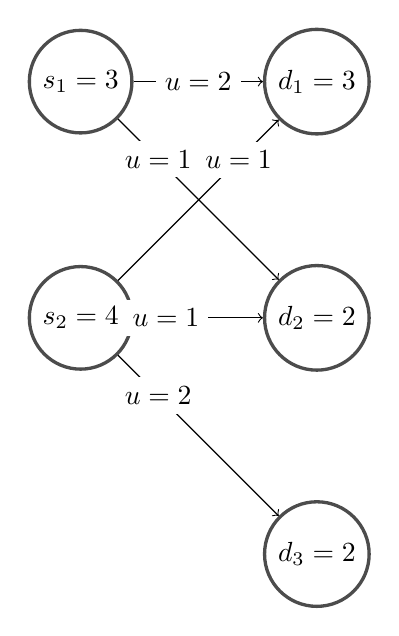
\begin{tikzpicture}[
node/.style={circle, draw=black!70, fill=white!5, very thick, minimum size=9mm}
]
%Nodes
\node[node]      (s1)                                        {$s_1= 3$};
\node[node]      (s2)     [below of =s1, yshift= -2cm]       {$s_2 = 4$};
\node[node]      (d1)     [right of =s1 , xshift= 2cm]       {$d_1 = 3$};
\node[node]      (d2)     [below of = d1, yshift= -2cm]       {$d_2 = 2$};
\node[node]      (d3)     [below of = d2, yshift= -2cm]      {$d_3 = 2$};
%Lines
\draw[->] (s1) -- (d1) node [midway, fill=white] {$u=2$};
\draw[->] (s1) -- (d2) node [near start, fill=white] {$u=1$};
\draw[->] (s2) -- (d1) node [near end, fill=white] {$u=1$};
\draw[->] (s2) -- (d2) node [near start, fill=white] {$u=1$};
\draw[->] (s2) -- (d3) node [near start, fill=white] {$u=2$};
\end{tikzpicture}
\caption{At this point, there are no more reduced cost cylces, so we've found an optimal solution in terms of cost. The edges reflect the amount of units flowing from supply to demand in this solution.}
\label{fig:example5}
\end{framed}
\end{figure}

\begin{figure}
\centering
\begin{framed}
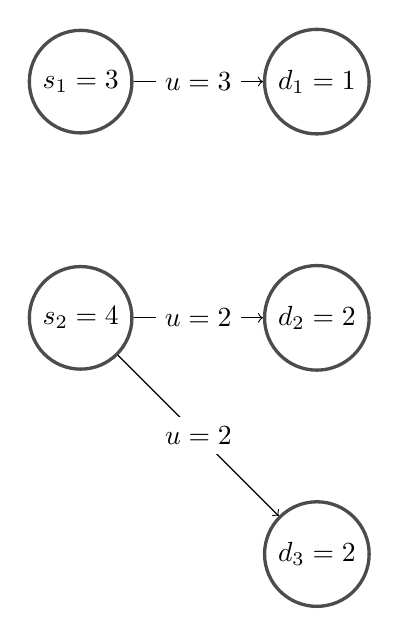
\begin{tikzpicture}[
node/.style={circle, draw=black!70, fill=white!5, very thick, minimum size=9mm}
]
%Nodes
\node[node]      (s1)                                        {$s_1= 3$};
\node[node]      (s2)     [below of =s1, yshift= -2cm]       {$s_2 = 4$};
\node[node]      (d1)     [right of =s1 , xshift= 2cm]       {$d_1 = 1$};
\node[node]      (d2)     [below of = d1, yshift= -2cm]       {$d_2 = 2$};
\node[node]      (d3)     [below of = d2, yshift= -2cm]      {$d_3 = 2$};
%Lines
\draw[->] (s1) -- (d1) node [midway, fill=white] {$u=3$};
\draw[->] (s2) -- (d2) node [midway, fill=white] {$u=2$};
\draw[->] (s2) -- (d3) node [midway, fill=white] {$u=2$};
\end{tikzpicture}
\caption{As long as there aren't minimum cost cylces we've found a solution. Zero-cost cycles exists in this simple network. As a result, there is more than 1 solution that optimizes cost and flow. This figure shows that example.}
\label{fig:example6}
\end{framed}
\end{figure}

\section{Linear Programming}

\subsection{The Simplex Algorithm}

There are a few ways to solve this problem. Because I have a lot of variables I want to solve for, I plan on specifying this problem as linear program and solving it with the simplex algorithm. This algorithm is essentially like the ordinary least squares of optimization. People have written textbooks describing it's properties and variation. A quick google search would do a better job of explaining than me, but I'll try any way. The algorithm finds the solution to a linear objective (i.e. $a x_1 +b x_2 + ...$ ) subjected to linear constraints. The intuition behind how it works is that it states the problem in two ways and finds the lowest maximum and highest minimum. When these happen to coincide,  you know you've found a maximum. At first glance, the  linear nature of the problem function might look like OLS, but they are very different. In OLS, the estimated coefficinets are used to approximate some variable of interests. In linear programming, you get point values for each of the variables of interest to minimize the objective function.

\subsection{Primal Problem}

In order to use linear programming packages, we need to formally state the problem. The statement is fairly intuitive. As we said before, the problem tries to send as much units of a good from a suppliers $s$ in the set $S$ to demanders $d$ in the set $D$. However, there are costs for sending a unit of good across every route between suppliers and demand-ers. We want to minimize these costs which leads to our objective function (in the objective $c$ is costs and $u$ is units of the good).

$$\operatorname{Minimize} \sum_{s,d \in \text{Routes}} c_{s,d} u_{s,d}$$

The constraints on the objective function reflect the fact that supply and demand must should balance. The first set of contraints require that demand be satisfied.

$$\sum_{s,d \in \text{Routes}} \text{u}_{s,d}= \text{demand at } d \text{ (for all demand-ers } s \in S)$$

The second set of constraint requires that no supply goes to waste. In other words, no product is just left at suppliers. In this case, supply is a negative quantity because supply leaves the supply nodes and flows to demand nodes.

$$\sum_{s,d \in \text{Routes}} \text{u}_{s,d}= \text{supply at } s \text{ (for all suppliers } d \in D)$$

Finally, we can't have negative amounts of units flow across the routes.

$$0 \leq u_{s,d}, \forall s,d \in \text{Routes}$$

Putting it all together, supply in demand balance because suppliers are required to send a certain amount of flow and demand-ers must receive a certain amount.
$$\operatorname{Minimize} \sum_{s,d \in \text{Routes}} c_{s,d} u_{s,d}$$
$$\text{subject to}$$
$$\sum_{s,d \in \text{Routes}} \text{u}_{s,d}= \text{demand at } d \text{ (for all suppliers } s \in S)$$
$$\sum_{s,d \in \text{Routes}} \text{u}_{s,d}= \text{supply at } s \text{ (for all demand-ers } d \in D)$$
$$0 \leq u_{s,d}, \forall s,d \in \text{Routes}$$

To summarize, the objective function minimizes total costs. The first and second constraints ensure nodes either produce or consume based on their type; the third ensures supply moves forward from supply to demand.  In the case, when supply doesn't equal demand you can add an extra node to the problem. You let other nodes send supply or recieve goods from this node at 0 cost (depending on whether there is too much supply or demand). The amount flow from this node to others represents a shortage or surplus.


\subsection{Dual Problem}

Every linear program has an equivalent dual problem. In the dual, the constraints become the variables of interest and the variables of interest become constraints. I used the dual problem to solve optimal transport because it yeilds a more interesting economic interpretation. The dual variables can be interpretted as optimal prices from a social planning perspective.

The intuition behind the dual problem for optimal transport comes from the desire to get rid of augmenting cycles. The dual formalizes this idea. Essentially we introduce a slack variable at each node $p$. When we compute the costs of cycles we can trivially add and subtract $p$ at each node. As long as the slack variables cancel we haven't changed the nature of the problem. However, since this is a slack variable, it can take what ever value we want. We can use the difference between $p_d$ and $p_s$ to encode the maximum amount we can reduce the cost of crossing the edge from suppler $s$ to demand-er $d$ for one unit of goods. For this reason, in the optimal solution we want to

$$\operatorname{Maximize} \sum_{d \in D}  (\text{demand at } d) \cdot p_{d} -   \sum_{s \in S}  (\text{supply at } s) \cdot p_{s} $$

Here we're trying to maximize the difference between all the $p$'s at the demand nodes and all the $p$'s at the supply nodes. We need to scale $p$ at each node in the object to reflect the fact multiple units will be sent from $s$ to $d$. We wouldn't accomplish anything special if we only considered sending one unit across. Essentially this is trying to eliminate all possible reduced cost cylces.

The consraints in the dual variable reflect the fact that you can only reduce the cost across an edge so much. At a certain point, you must incur some cost for traversing an edge. This is expressed formally as

$$ p_d -p_s  \leq c_{s,d}$$

Putting it together we have

$$\operatorname{Maximize} \sum_{d \in D}  (\text{demand at } d) \cdot p_{d} -   \sum_{s \in S}  (\text{supply at } s) \cdot p_{s} $$
$$ \text{ subject to}$$
$$ -p_s + p_d \leq c_{s,d}, \forall s,d\in \textrm{Routes}$$


It helps to think of the dual variable as a price. Firms $s$ earns $p_d$ for sending their product to $d$ but looses $p_s + c_{s,w}$. The constraint prevents arbitrage through the network. If it didn't hold, all the firms would send their product across this edge. It's important to remember that when calculating the cost of a cylce through the network $p_d$ and $p_s$ will cancel. 

Thinking about the dual problem like a price also yields a more interesting economic description of the system. Basically, instead of finding the amount of units sent between each pair of suppliers and demand-ers, we can look prices that reflect the relative cost of sending goods to certain demanders. The dual variable $p_v$ can be interpreted as optimal prices from a social planning perspective. The problem maximizes profits from a social planning perspective. The constraint that arbitrage profits do not exist in the network. The price you pay at the demand node $p_d$, cannot exceed the price you pay at the supplier $p_s$ plus the cost of sending the unit of good $c_{d,s}$. This has to do with the fact that the algorithm completes when the reduced costs cycles are exhausted.

\subsection{Characterizing Solutions with Complementary Slackness}

From an economic perspective, I would hope you are skeptical of any solution to this problem involving prices found by the simplex algorithm. Optimal transportation can have more than one possible solution. The example I've worked out the problem actually has more than one solution and I've demonstrated it in Figure \ref{fig:example6}. The question becomes how do I know when I've found all possible minimum cost flow distributions through the network with the simplex algorithm. Perhaps I got lucky and found an interesting solution with certain properties that aren't robust.

Luckily, linear programming has a property that allows me to characterize all possible solutions. This property is called complementary slackness and it says that the optimal value of the primal and the dual objective functions will be equivalent. The intuition behind this idea is relatively easy to show with some matrix algebra.

Very generally speaking a linear program has the primal form

$$\text{Maximize } c' x$$
$$\text{Subject to}$$
$$Ax \leq b$$

And, it's corresponding dual would be

$$\text{Minimize } y' b$$
$$\text{Subject to}$$
$$A'y \leq c$$

We can massage the objective function to see that the values of the primal and dual objective functions will be the same

$$(A'y)' \leq c'$$
$$ y'A \leq c'$$
$$ y'Ax \leq c'x$$
$$y' b \leq c'x$$

In the same vain, 

$$ Ax \leq b$$
$$ y'Ax \leq y'b$$
$$ (yA')'x \leq c'x$$
$$ c'x \leq  y' b $$

As consequence of these two observations we know the objective functions must take the same value.

$$c'x = y' b$$

By this logic the objective funciton for any solution to the primal or dual problem will be the same. You can use this idea to check how robust certain properties of your solution are by limiting the linear program with the value of the objective function as a constraint. 

For example, in regards to the transporttion if you want to check to see whether your maximum price $p = p^{max}$ is only particular to your solution, you can add constraint extra constraints to your original problem to test this. You can request that one of the prices exceeds the maximum, $p > p^{max}$ to check this property of the solution. And, in order to ensure that this is still a valid solution to the original problem you can limit the value of your objective function. If the value of the objective was $c^*$ then you can add the constraint  $ \sum_{d \in D}  (\text{demand at } d) \cdot p_{d} -   \sum_{s \in S}  (\text{supply at } s) \cdot p_{s} = c^*$
 
\subsection{Computational Complexity}
It's worth mentioning is the efficiency of the simplex algorithm (i.e. computational complexity). Since, this is an economics honors thesis, I want to make it clear what I mean by this. Measuring a programs efficiency by factors like how long it takes to run or how many lines of code it takes can vary with the computer and the compiler. It is also variable with the input to the program. As a result, in order to have a more universal measure of efficiency the efficiency of algorithms are measured using run time bounds. Run time bounds are an upper bound on the number of steps you need to solve the problem, given the input. The simplex algorithm's run time bound is actually very bad as far as we know. It can be $O(2^n)$. Meaning that if there could be some scalar multiple of $2^n$ steps if there are $n$ input variables. However, in practice the simplex algorithm does much better. The general rule of thumb is that the simplex algorithm has a run time bound that is some polynomial of $n$ \cite{Cook}.


\chapter{Problem Specification}

\section{Explanation of the Problem}

Now that I've explained the machinery I'll be using, I want to explain the application. I've modeled the supply network for cherries, onions, cabbages, and grapes in New York using optimal transportation.  In my model, farms send their goods to intermediaries and which in turn send their crop to stores purely based on transportation cost. Exports are assumed to be insignificant. Farms, intermediaries, and vendors incur transportation costs equals to the expected travel time between them. Farms can ship to any intermediary associated with the same crop and intermediaries can ship to any store. Intermediaries can scale as much as they desire. Farms produce agricultural products proportional to their size. Stores satisfy demand proportional to the market value of their square footage. By modeling these crops using this framework, I can estimate prices for various regions in New York with the problem. These prices reflect a sort of relative cost for sending that crop to that region. I've drawn a picture of what this network looks like Figure \ref{fig:spec}.

\begin{figure}
\centering
\begin{framed}
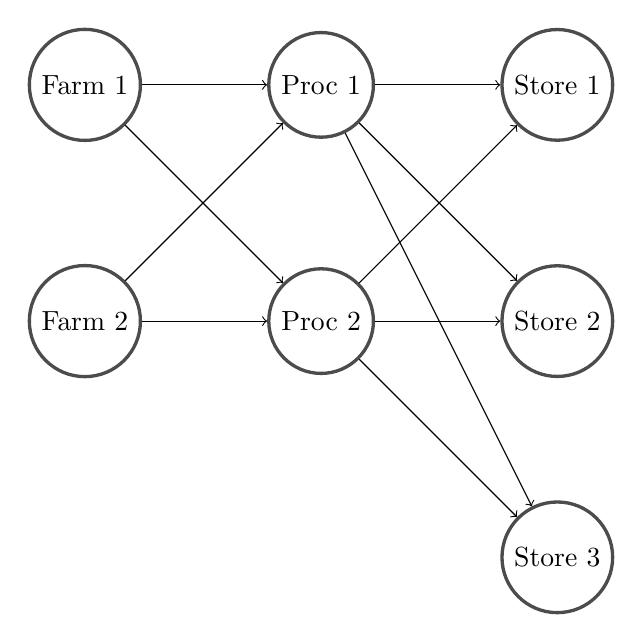
\begin{tikzpicture}[
node/.style={circle, draw=black!70, fill=white!5, very thick, minimum size=9mm}
]
%Nodes
\node[node]      (f1)                                        {Farm 1};
\node[node]      (f2)     [below of = f1, yshift= -2cm]       {Farm 2};
\node[node]      (p1)    [right of = f1, xshift= 2cm]        {Proc 1};
\node[node]      (p2)     [below of =p1, yshift= -2cm]       {Proc 2};
\node[node]      (s1)     [right of = p1 , xshift= 2cm]       {Store 1};
\node[node]      (s2)     [below of = s1, yshift= -2cm]       {Store 2};
\node[node]      (s3)     [below of = s2, yshift= -2cm]      {Store 3};
%Lines
\draw[->] (f1) -- (p1) ;%node [midway, fill=white] {};
\draw[->] (f1) -- (p2) ;%node [near start, fill=white] {};
\draw[->] (f2) -- (p1) ;%node [near start, fill=white] {distance};
\draw[->] (f2) -- (p2) ;%node [midway, fill=white] {distance};
\draw[->] (p1) -- (s1) ;%node [midway, fill=white] {distance};
\draw[->] (p1) -- (s2) ;%node [near start, fill=white] {distance};
\draw[->] (p1) -- (s3) ;%node [near end, fill=white] {distance};
\draw[->] (p2) -- (s1) ;%node [near end, fill=white] {distance};
\draw[->] (p2) -- (s2) ;%node [midway, fill=white] {distance};
\draw[->] (p2) -- (s3) ;%node [near start, fill=white] {distance};
\end{tikzpicture}
\caption{This figure show the structure of the agricultural supply network in my model. Farms grow crops and send their product to intermediate processors. Processors send their product to stores. The processors and farms send their product to the next step in the network using local roads. They choose where to send their crops based on convenience.}
\label{fig:spec}
\end{framed}
\end{figure}

This is actually a pretty reasonable way to think about New York agriculture for certain crops. Specifically, the crops I plan to model in this way are cabbage, onions, grapes and cherries. Production of these crops largely falls into three stages. First, farms produce crops (i.e. they are suppliers). Then they send their goods to intermediaries called agricultural dealers. The agricultural dealers may do some intermediate processing (like putting to produce in bags), but they largely leave the produce alone. After they are done, intermediaries in turn send their crop to stores (i.e. demand-ers). The stores in turn allow consumers to buy the crop. Since the products are not exported on a large scale and have relatively short shelf life, supply largely equals demand (although it is possible to include exports in the model). Additionally this means that firms choose where to send their product based on convenience. In other words, it seems reasonable to say that farms, intermediaries, and vendors want chose where to send their goods by minimizing the costs. 

\section{Reduction to Linear Program}

Assuming I can measure demand, supply, and the edge costs in the network, I can reduce the problem I've described to optimal transporation. By reduce, I mean I want to show that the problem I've specified above can be  written as a linear 
program which I can solve with the simplex algorithm. In this section, I will be formally explaining the way I did this.

\subsection{Primal Problem Formulation}
It is easy to see that problem for my agricultural networks is essentially the same as minimum cost flow. Farms are suppliers and stores are demand-ers. Supplies and demands balance because these crops are not really exported. The only difference is the inclusion of processors. Farms can send produce to which ever processor they like and processors can send produce to which ever store they like. However, farms cannot send their produce straight to the stores. The objective function is updated to reflect this change. Farms must incur the cost of sending their goods to processors, and stores incur the cost of recieiving their goods from processors (instead of just sending goods between farms and stores like the original problem).

$$\operatorname{Minimize} \sum_{f,p \in \text{Routes}} c_{f,p} u_{f,p} + \sum_{p,s \in \text{Routes}} c_{p,s} u_{p,s}$$

We also need to add an additional constraint onto the processors in the linear program. This constraint prevents the processors from keeping any of the crops.

$$\sum_{f,p \in \text{Routes}} \text{u}_{f,p} + \sum_{p,s \in \text{Routes}} \text{u}_{p,s} = 0 \text{ (for all processors } p \in P)$$

So, putting everything together we specify the primal problem:

$$\operatorname{Minimize} \sum_{f,p \in \text{Routes}} c_{f,p} u_{f,p} + \sum_{p,s \in \text{Routes}} c_{p,s} u_{p,s}$$
$$\text{subject to}$$
$$\sum_{f,p \in \text{Routes}} \text{u}_{f,p}= \text{supply at } f \text{ (for all farms } f \in F)$$
$$\sum_{f,p \in \text{Routes}} \text{u}_{f,p} + \sum_{p,s \in \text{Routes}} \text{u}_{p,s} = 0 \text{ (for all processors } p \in P)$$
$$\sum_{p,s \in \text{Routes}} \text{u}_{p,s}= \text{demand at } s \text{ (for all stores } s \in S)$$
$$0 \leq u_{s,d}, \forall s,d \in \text{Routes}$$

So to summarize, we are minimizing the cost of sending goods from farms to processors and processors to stores. In the problem, we are imposing the constraints that farms send all the crops they grow, stores consume all the crops they recieve and processors do not keep any crops. This is essentially optimal transport.

\subsection{Dual Problem Formulation}

Of course, I am interested in prices, or more accurately relative transportation costs. As a result, I will be solving the dual problem, not the primal one. As I explained before, the dual variable represents a sort of price that incentivizes firms to send their product across certain edges. The dual problem's objective stays exactly the same as before.

$$\operatorname{Maximize} \sum_{s \in S}  (\text{demand at } s) \cdot p_{s} -   \sum_{f \in F}  (\text{supply at } f) \cdot p_{f} $$

Since, we've added processors into the primal's objective function we now need two sets of constraints, one for the edges between the farms and processors, and another for the edges between the processors and stores. They essentially prevent every farm from sending their goods to a certain processor and processors from sending all their goods to a certain store. The constraints say that  the price at the source plus the edge cost must outweigh the cost at the destination (just like before).

$$ -p_f + p_p \leq c_{f,p}, \forall f,p\in \textrm{Routes}$$
$$ -p_p + p_s \leq c_{p,s}, \forall p,s\in \textrm{Routes}$$

Putting everything together we have our dual problem:

$$\operatorname{Maximize} \sum_{s \in S}  (\text{demand at } s) \cdot p_{s} -   \sum_{f \in F}  (\text{supply at } f) \cdot p_{f} $$
$$ \text{ subject to}$$
$$ -p_f + p_p \leq c_{f,p}, \forall f,p\in \textrm{Routes}$$
$$ -p_p + p_s \leq c_{p,s}, \forall p,s\in \textrm{Routes}$$

\section{Data Sources}

Now that I've specified my problem as a linear program, the next question is how quantify supply at farms, demand at stores, and the edge costs. To measure supply I use the pixels in a a sattelite image of crop cover.  To measure measure demand, I use the square footage of each store weighted by median household prices nearby. These crop are mostly grown to satisfy in state demand because of their relatively shorter shelf life a smaller scale production. As a result, I measured supply and demand as proportions of the total (to ensure they balance). To measure the edge costs, I use open source routing software to find the expected travel time. Obviously, empirical data is never perfect, but the datasets I found do a good job at capturing the essence of the problem.

\subsection{Farms}

In the final linear program, each farm's supply was its proportion of the total amount of area. In general, land cover is highly proportional to yeilds especially for the same crop. Considering these farms are fairly close, they face roughly the same geographic conditions and weather. Unless farmers have access to drastically different technologies, the biggest difference affecting yeilds for farms is area.

My data on area and location came from an image created by the National Agricultural Statistical Service \cite{nass}. It is called the Cropland Data Layer (CDL). The file is created by measuring the way light reflects off the Earth at certain wavelengths using a Sattelite (Landsat). The sattelite measures this reflection at $30 \times 30$ square meter plots. Based on the reflection is possible to classify point measured by the sattelite. The classifications are made using training data from the Farm Service Agency (FSA) Common Land Unit (CLU) Program and non-agricultural training data from the United States Geological Survey (USGS) National Land Cover Dataset 2001 (NLCD 2001) The final product is a file forms a grid called a raster. Pixels in the image represent certain crop bands. The accuracy of classification for these pixels isn't great. In Table \ref{tab:band}, you can see how accurate the sattelite data is. 

\begin{table}
\centering
\begin{framed}
\begin{tabular}{c|c|c|c|c|c}%
	Type&Band&Correct Pixels&Producer's Accuracy&Kappa&User's Accuracy
    \csvreader[head to column names]{band.csv}{}% use head of csv as column names
    {\\\hline \csvcoli & \csvcolii & \csvcoliii & \csvcoliv& \csvcolv & \csvcolvi}
\end{tabular}
\caption{This table shows the various errors associated with pixels in each crop band in the sattelite image. The pixels are compared with a small test set for accuracy. Correct pixels are the number of pixels extrapolated from the training data. Producer's accuracy is a false negative, where pixels of a known class are classified as something other than that class. User's accuracy shows false positives, where pixels are incorrectly classified as a known class when they should have been classified as something else. Kappa index of agreement gives an overall assessment of the accuracy of the classification.}
\label{tab:band}
\end{framed}
\end{table}

Although individual pixels may be unreliable, I am counting on the fact that clusters of pixels do actually correspond to the locations of farms. Since, I was interested in the area taken up by farms, I used a technique called seiving to make the image more uniform and get rid of random pixels. Basically, this technique involves identifying clusters of continuous pixels and dropping the pixels in clusters smaller than a certain size. After creating the seive, I converted the raster file into vector based polygons to calculate the area of each cluster and the centroid. Each cluster of continuous pixels became a farm with an area and a centroid. To give you a sense of what farms looked like across the various bands I've included Figure \ref{tab:farms}. You can see how farms for each band look (and how an explnation of how the shapes related to the results) in the results section.


\begin{table}
\centering
\begin{framed}
\begin{tabular}{c|c|c|c|c|c}%
	Band&Total&Average&Minimum&Maximum&Variance
    \csvreader[head to column names]{farms.csv}{}% use head of csv as column names
    {\\\hline \csvcoli & \csvcolii & \csvcoliii & \csvcoliv& \csvcolv & \csvcolvi}
\end{tabular}
\caption{This table is meant to summarize some statistics of interest about the size of farms. Some take aways are that onions (band 49) take up the most area followed by grapes (band 69). Cabbages (band 243) have the smallest range of sizes, but the highest variance within that range. Cherries (band 66) have the smallest variance and the smallest total cover.}
\label{tab:farms}
\end{framed}
\end{table}


\subsection{Agricultural Product Dealers}

In order to include intermediate processors (i.e. the Agricultural product dealers) into the problem, I used the data on permits from the NYS Department of Agricultural Markets \cite{dam}. Basically, the state keeps a list of all the businesses that buy more than 10,000 dollars in agricultural products. The data set had information about the crops they sold, and their location as an address. I converted the addresses to a spatial coordinate using Nominatim, an open source platform for geolocating (i.e. converting addresses into cooridnates). There are roughly 300 of them, but only half were relevant to my problem because they sold the right type of crop. I've included Table \ref{tab:procs} to give you a sense of how many processors were associated with each crop band.

I've included the processors in the problem for two reasons. For starters, they make the problem more realistic by adding limitations to where the farms can sell product. I made sure to choose bands where (for the most part) produce isn't drastically altered during intermediate processing. If the crops make it to these dealers they are going to be sold to stores then consumed. This is because these dealers don't have the necessary permits to use the produce for a purpose other than resale. Only 2 of the 300 processors were from out of state. New York is much bigger on exporting dairy than produce. Obviously, the dealers can sell it to businesses that make prepared foods. For example, a certain percentage of grapes make juices and wine. In practice, the business that with the necessary permits buy in bulk from farms. 

The second reason for including the dealers is because they number of edges to make the problem more computationally tractable. There were roughly 300 licensed agricultural product dealers in the data set. By forcing the edges between stores and farms to the processors, I drastically cut down the number of edges. 


\begin{table}
\centering
\begin{framed}
\begin{tabular}{c|c}%
	Band & Count
    \csvreader[head to column names]{procs.csv}{}% use head of csv as column names
    {\\\hline \csvcoli & \csvcolii}
\end{tabular}
\caption{Grapes (band 69) has the highest number of product dealers associated with them. The lowest is cherries (band 66).}
\label{tab:procs}
\end{framed}
\end{table}


\subsection{Stores}

The data I used on stores came from NYS Division of Food Safety. It is essentially the list of stores that are given health inspections. The store data set has roughly 20,000 different stores, the classifications are based on their permits, their square footage, and their location (as a GPS coordinate). I choose to look at the classification 'JAC' which are vendors that are registered as stores, manufacturers and multiple operations. This is because grocery stores fall under this category. Other categories were not as common and less relevant to selling fresh produce. I've included a map to give a sense of how they are spread through out the state in Figure \ref{fig:map_3}. To get a sense of how the stores vary in size, I've included Table \ref{tab:stores}.

\begin{figure}
\centering
\begin{framed}
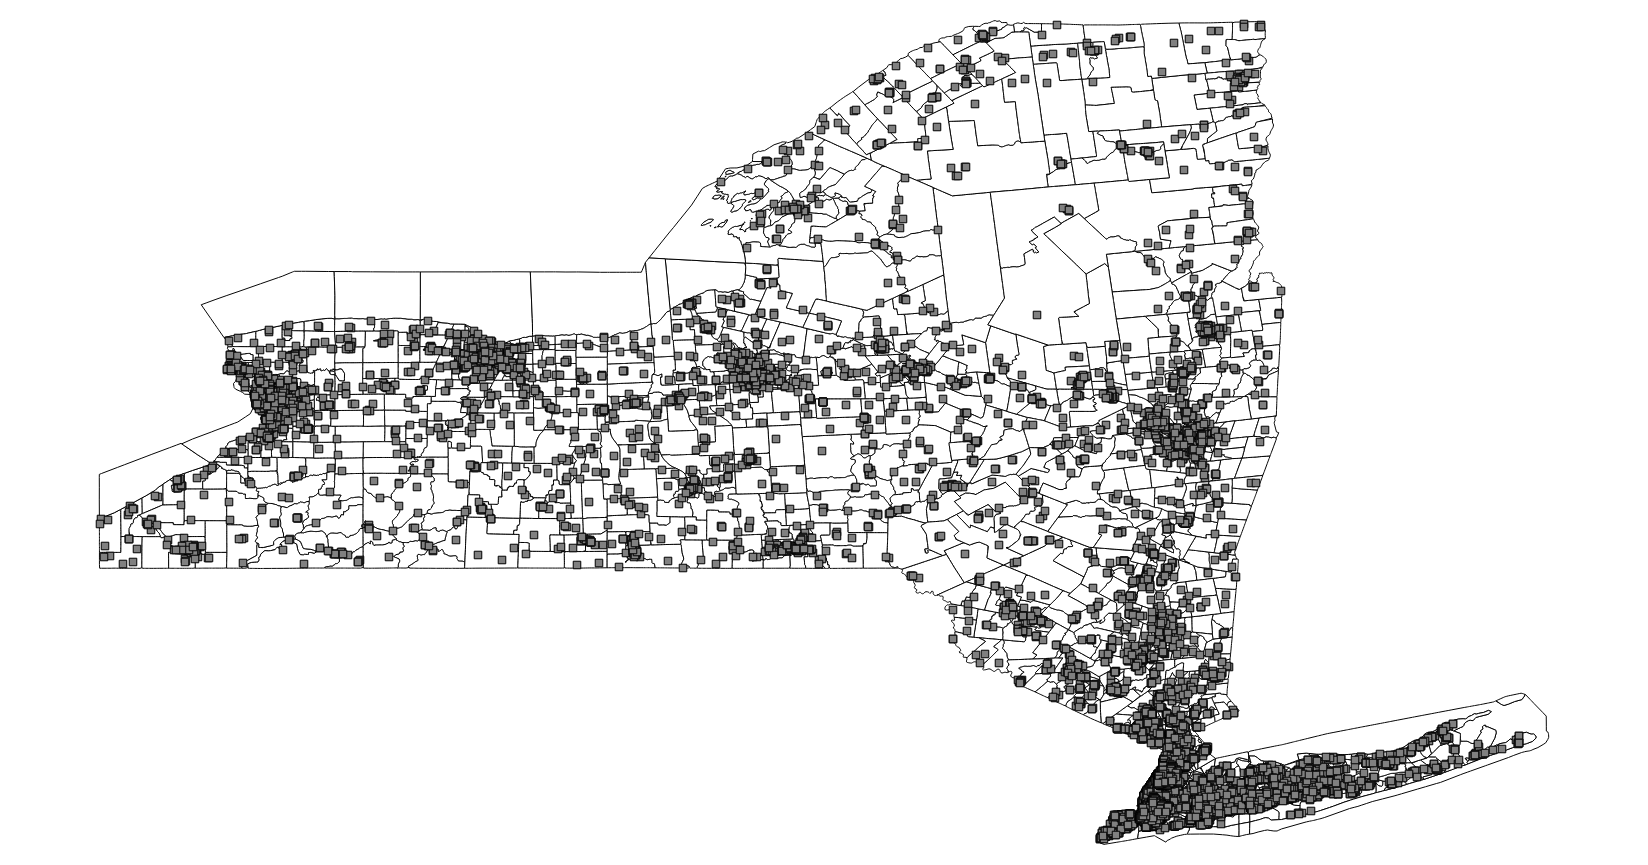
\includegraphics[scale=.4]{map_3}
\caption{Here I've mapped all the stores as grey squares. They've been overlayed on top of the census tracts so you can see that stores are spread out between them. You can see are much more sparsely spread in the center of the state.}
\label{fig:map_3}
\end{framed}
\end{figure}

\begin{table}
\centering
\begin{framed}
\begin{tabular}{c|c|c|c|c}%
	Band&Average&Minimum&Maximum&Variance
    \csvreader[head to column names]{stores.csv}{}% use head of csv as column names
    {\\\hline \csvcoli & \csvcolii & \csvcoliii & \csvcoliv & \csvcolv}
\end{tabular}
\caption{This table is meant to convey summary statistics about the characteristics of stores.}
\label{tab:stores}
\end{framed}
\end{table}

So as not to have a ridiculous number of edges between the stores and the intermediaries, I've actually aggregated the number of edges by Census district. The reason for using this method to aggregate stores is because I am multiplying square footage of the stores by the property to more appropriately weight the value of the square footage (i.e. a store in New York City might be the same size as a store upstate, but it you might expect it to sell significantly more produce even though they are the same size. This is because the population density is much tighter in new york and the consumers might have more income to spend on produce in New York). You can see these weights in Figure \ref{fig:map_4}.

\begin{figure}
\centering
\begin{framed}
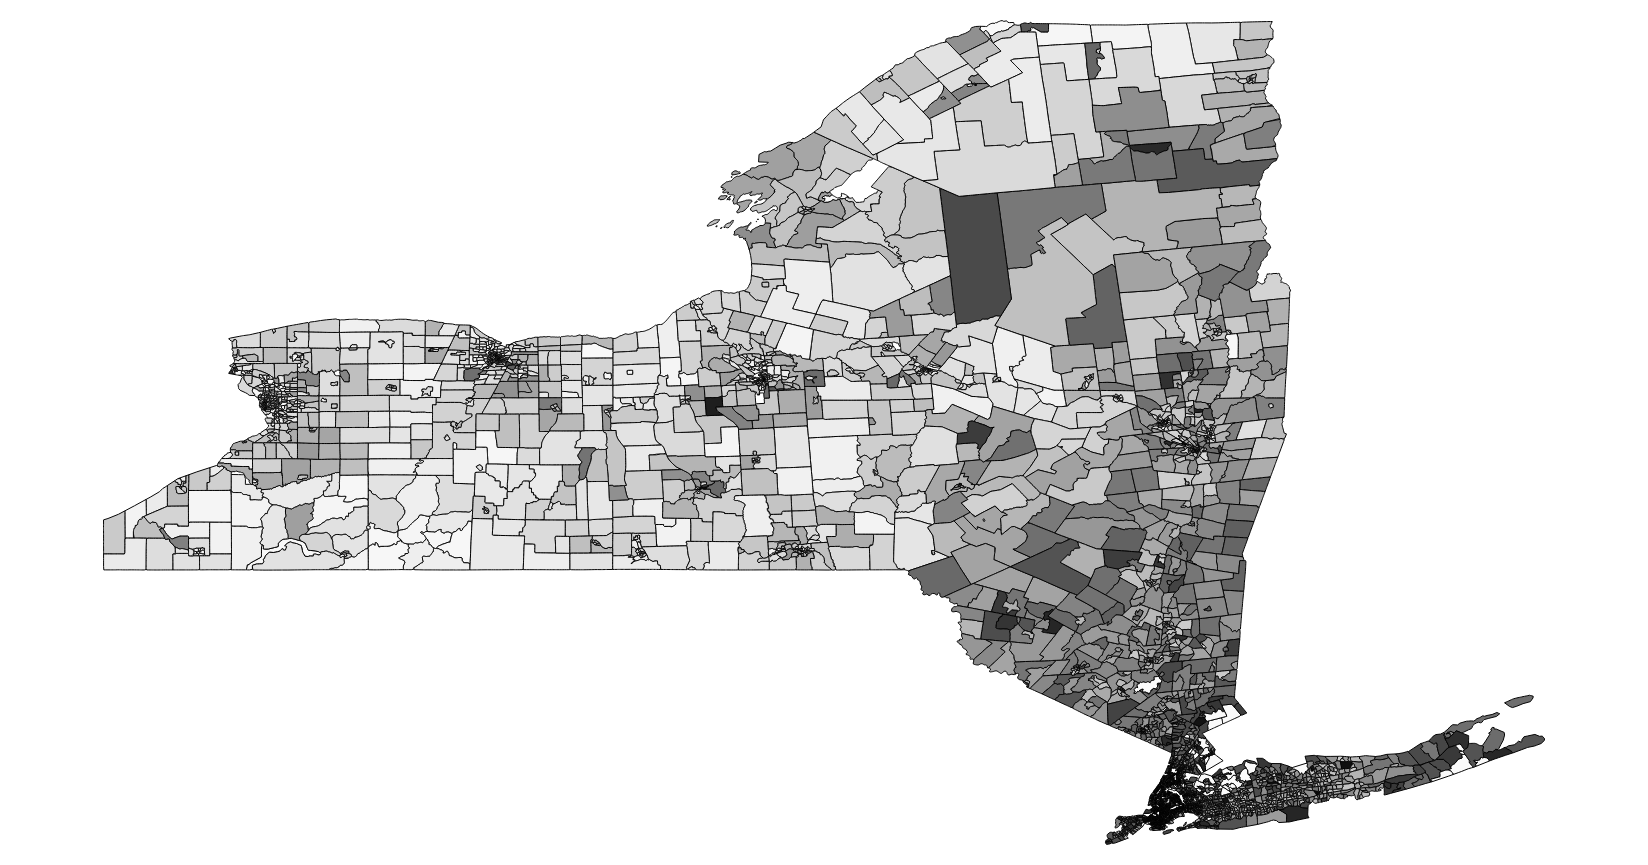
\includegraphics[scale=.4]{map_4}
\caption{The purpose of this map shows the distribution of median housing values through out the census tracts. The darker the shading, the higher the median property value for that tract. You can see housing is relatively cheap in western and Northern New York, but expensive in the South Western corner of the state.}
\label{fig:map_4}
\end{framed}
\end{figure}

I'm essentially assuming that when the stores choose how big they are, they value the properties based on how much they can how much one city versus anther translates into sales and they choose an optimal size appropriately. This is by no means meant to be an exact estimate and specifying a problem where store owners choose optimal square footage to meet demand would be a lot more complicated, it's only supposed to be better than a naive estimate of area by its self.

\subsection{Edge Costs}

In the model, I created an edge between every farm and every processor, and every processor and every store. I measured the cost of traversing this edge as the expected travel time in seconds. In order to find this number, I used open source software called open source routing machine (OSRM). The algorithm that OSRM implements is called contraction hierarchies. Essentially it is a technique to speed up shortest-path routing by first creating precomputed "contracted" versions of the connection graph. Contraction hierarchies can be used to generate shortest-path routes much more efficiently than the standard shortest path algorithm (i.e. Djisktra's). I downloaded a map from the open source mapping project (OSM) and answered routing queries over my local network about routing.

I've included two tables to give you a sense of some of the summary statistics of the edges. Table \ref{tab:fp_edges} shows the average, minimum, maximum, and variance of edges between farms and product dealers. Table \ref{tab:ps_edges} shows the same thing for the edges between dealers and stores.


\begin{table}
\centering
\begin{framed}
\begin{tabular}{c|c|c|c|c}%
	Band&Average&Minimum&Maximum&Variance
    \csvreader[head to column names]{fp_edges.csv}{}% use head of csv as column names
    {\\\hline \csvcoli & \csvcolii & \csvcoliii & \csvcoliv & \csvcolv}
\end{tabular}
\caption{This table is meant to convey summary statistics about the characteristics of the edges between farms and agricultural product dealers. Grapes (band 69) have the highest variability between edges. }
\label{tab:fp_edges}
\end{framed}
\end{table}

\begin{table}
\centering
\begin{framed}
\begin{tabular}{c|c|c|c|c}%
	Band&Average&Minimum&Maximum&Variance
    \csvreader[head to column names]{ps_edges.csv}{}% use head of csv as column names
    {\\\hline \csvcoli & \csvcolii & \csvcoliii & \csvcoliv & \csvcolv}
\end{tabular}
\caption{This table is meant to convey summary statistics about the characteristics of the edges between farms and agricultural product dealers. The distances are relatively similar to those of between farms and processors, but they are less variable}
\label{tab:ps_edges}
\end{framed}
\end{table}

\subsection{Implementing Optimal Transportation with Software Packages}

I'm a big believer in open source code. As a result, I've made all the code I wrote for this project publicly available on GitHub with a detailed explanation about how to get it running. It's mostly written in python, with a few SQL queries. Since open source is important to me, most of the software dependencies that need to be installed in order to get my code working are open source. The one exception is the linear optimizer. In this case, I used Gurobi which is free with an academic license. You can access the code at \url{http://github.com/erichschulman/ag_networks}.

\chapter{Results}


In order to make the result of the linear program understandable I've created a series of images of New York State. The big take aways from the result of the linear programming model is that the prices in Western part of the state are relatively low. The Southern corner and the North on the other had are significantly higher.  This finding results from the locations from farms within the state. Most farms are in the western part of the state. Additionally, when there are more farms that are smaller in size, it causes the variance in relative costs to go down through out the state. I've tested the robustness of these results by adding additional constraints to the objective function and using complementary slackness.


Of course the caveat to accepting these results is accepting that the linear program and my specification is not an excersize in futility. Even though the model is crude, the question is if it captures the most important aspects of what is going on. In terms of broader implcations for these results, the question is the degree to which transporation costs really influence prices of produce accross the state. This is a question that my model leaves un answered.

\section{Visualizing Results}

I've created a series of images to make the nature of the network for each crop and the result of the linear program intelligble. The images show farms, stores and dealers on the same map. They also show various census tracts with shading based on the relative magnitude of the prices. The actually number assigned to the price is some what irrelevant because they only have meaning in relation to each other. The prices created by the linear program aren't really prices. The are essentially relative costs due to transportation.

\subsection{Onion Farms}

Figure \ref{fig:price_49}

\begin{table}
\centering
\begin{framed}
\begin{tabular}{c|c|c|c}%
	Type&Average&Variance&Deviation
    \csvreader[head to column names]{price_49.csv}{}% use head of csv as column names
    {\\\hline \csvcoli & \csvcolii & \csvcoliii & \csvcoliv}
\end{tabular}
\caption{Another table caption}
\label{fig:price_49}
\end{framed}
\end{table}

\begin{table}
\centering
\begin{framed}
\begin{tabular}{c|c|c|c|c}%
	Type&Max Price&Max County&Min Price&Min County
    \csvreader[head to column names]{county_49.csv}{}% use head of csv as column names
    {\\\hline \csvcoli & \csvcolii & \csvcoliii & \csvcoliv & \csvcolv}
\end{tabular}
\caption{Another table caption}
\end{framed}
\end{table}

\begin{figure}
\centering
\begin{framed}
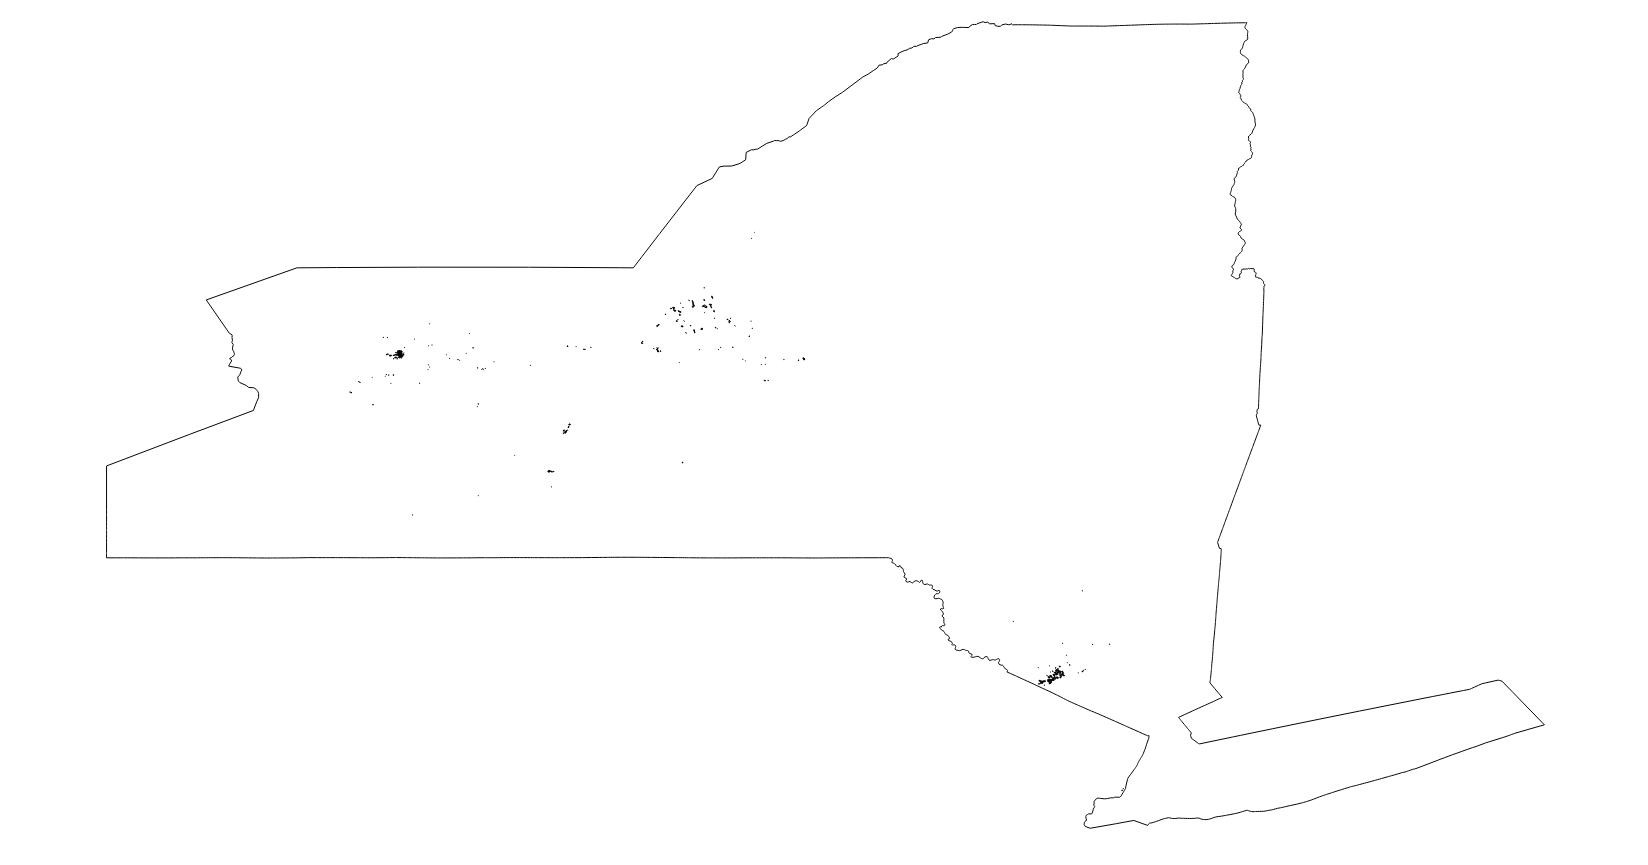
\includegraphics[scale=.4]{farms_49}
\caption{This shows something}
\label{fig:farms_49}
\end{framed}
\end{figure}

\begin{figure}
\centering
\begin{framed}
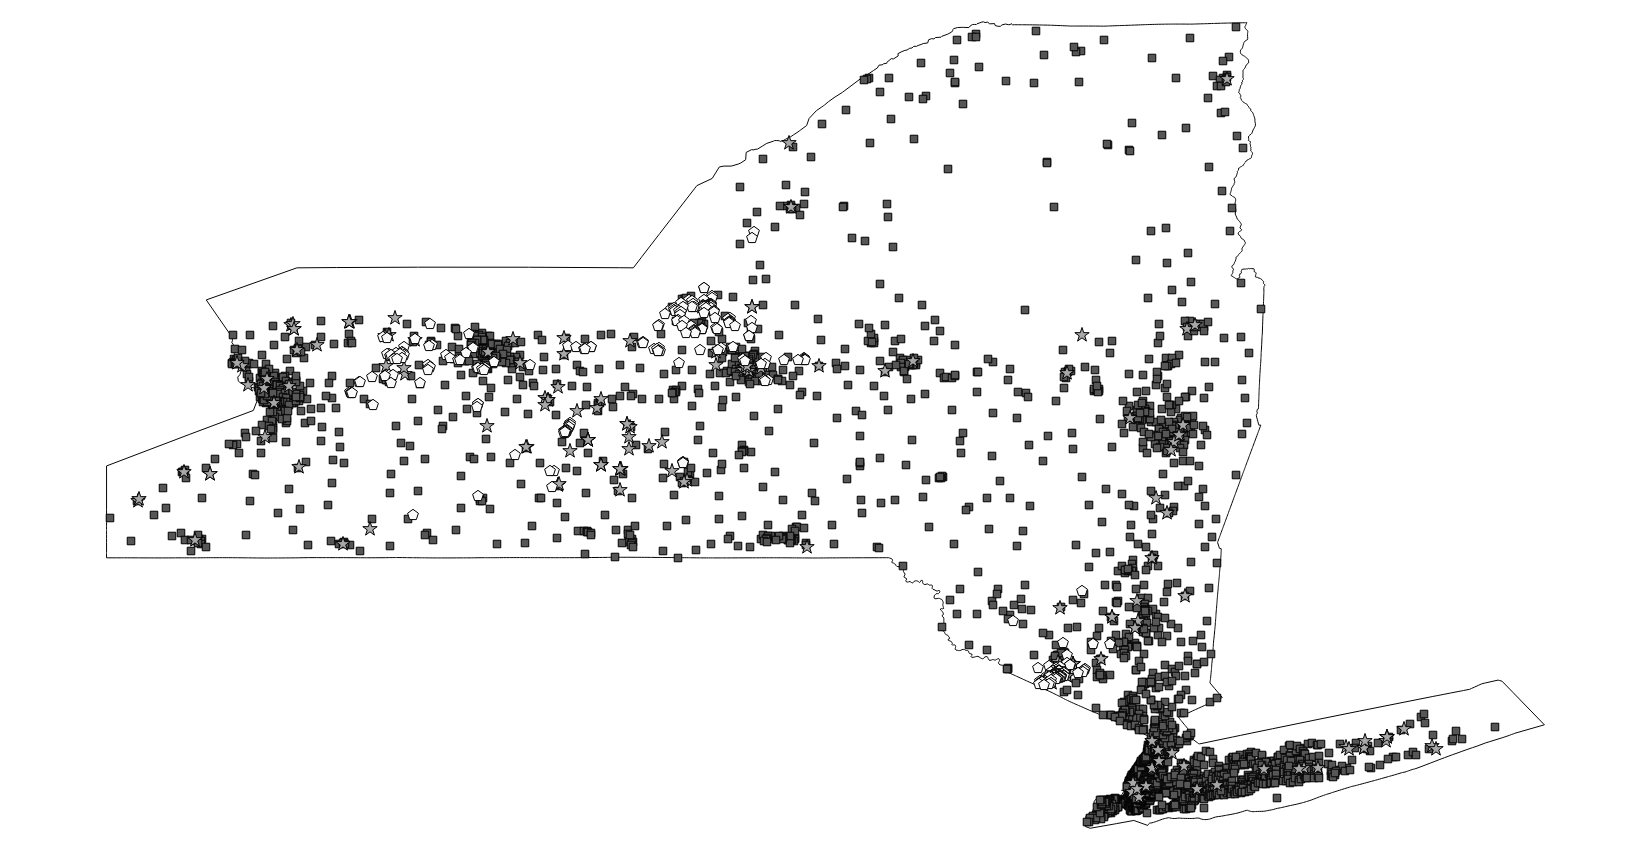
\includegraphics[scale=.4]{network_49}
\caption{This shows something}
\end{framed}
\end{figure}

\begin{figure}
\centering
\begin{framed}
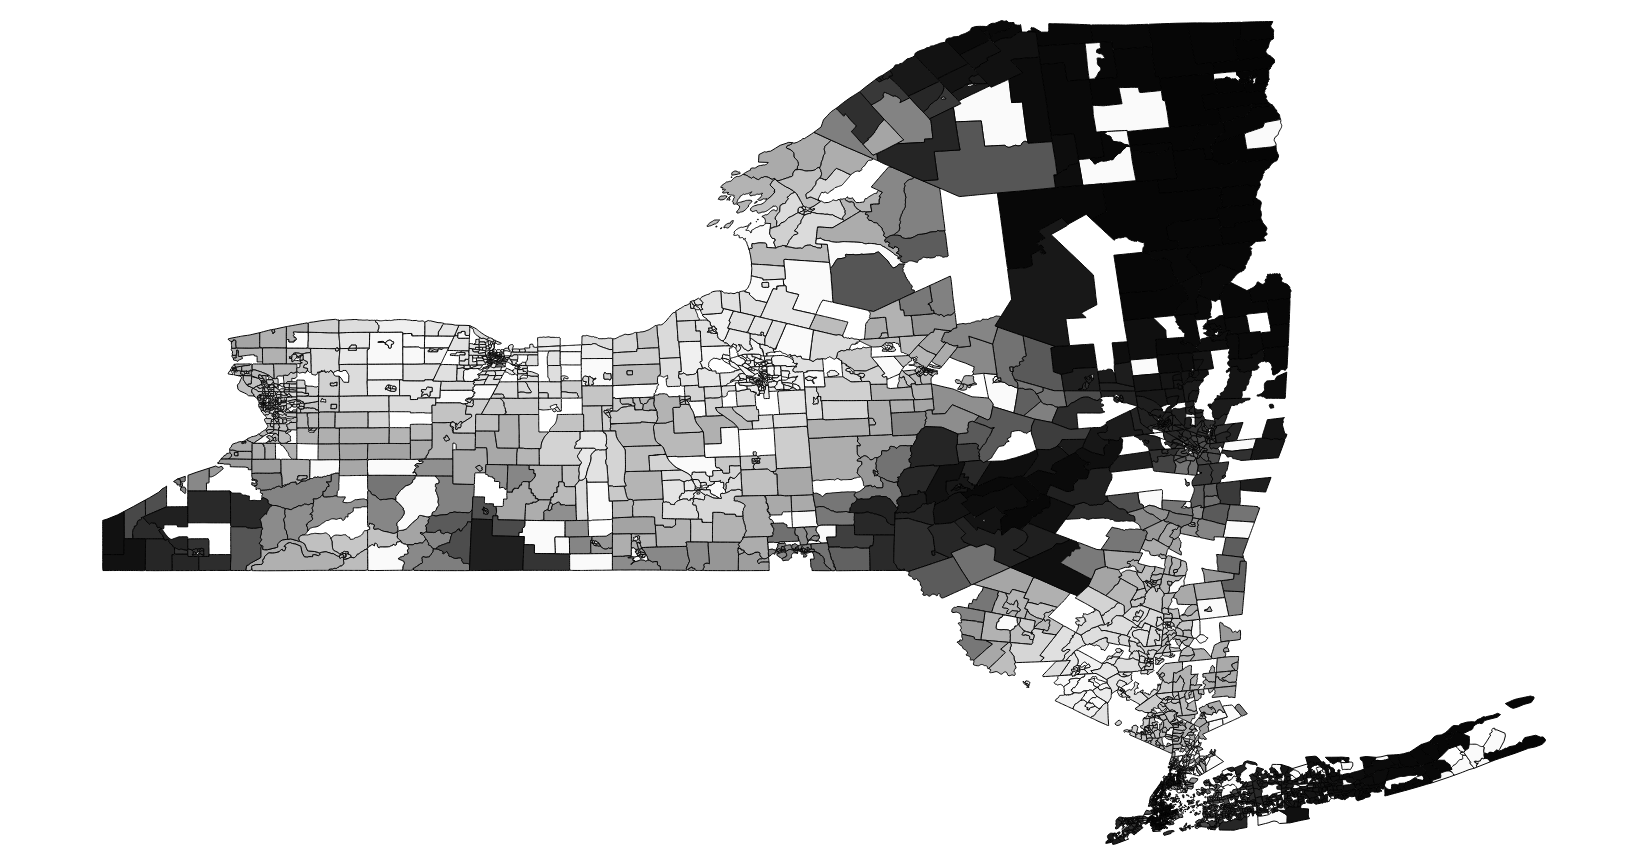
\includegraphics[scale=.4]{prices_49}
\caption{This shows something}
\end{framed}
\end{figure}

\subsection{Cherry Farms}

\begin{table}
\centering
\begin{framed}
\begin{tabular}{c|c|c|c}%
	Type&Average&Variance&Deviation
    \csvreader[head to column names]{price_66.csv}{}% use head of csv as column names
    {\\\hline \csvcoli & \csvcolii & \csvcoliii & \csvcoliv}
\end{tabular}
\caption{Another table caption}
\end{framed}
\end{table}

\begin{table}
\centering
\begin{framed}
\begin{tabular}{c|c|c|c|c}%
	Type&Max Price&Max County&Min Price&Min County
    \csvreader[head to column names]{county_66.csv}{}% use head of csv as column names
    {\\\hline \csvcoli & \csvcolii & \csvcoliii & \csvcoliv & \csvcolv}
\end{tabular}
\caption{Another table caption}
\end{framed}
\end{table}

\begin{figure}
\centering
\begin{framed}
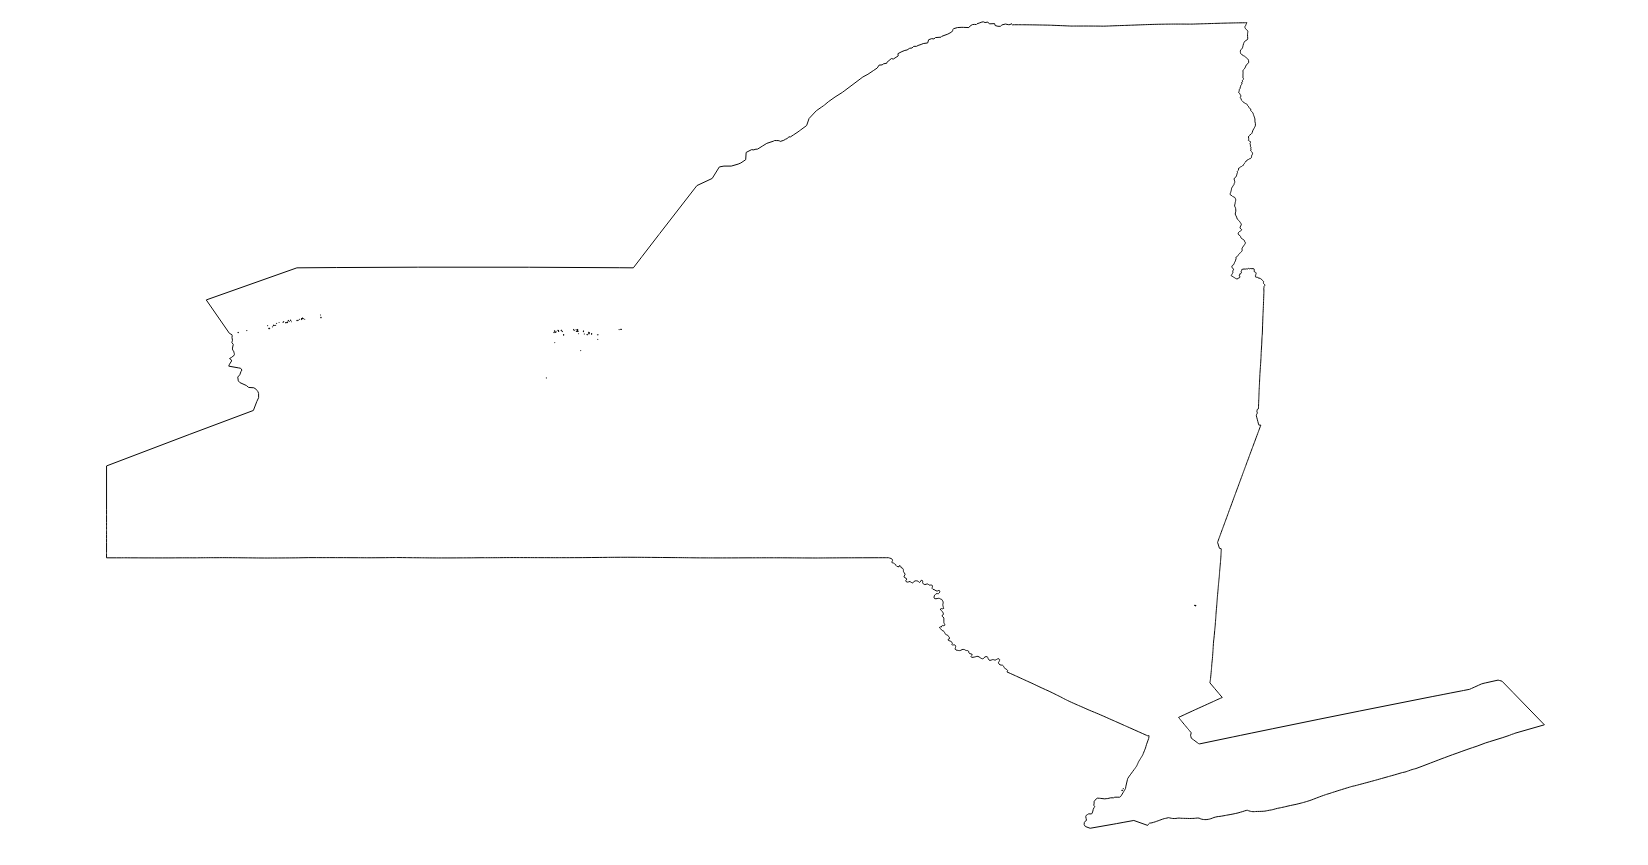
\includegraphics[scale=.4]{farms_66}
\caption{This shows something}
\label{fig:farms_66}
\end{framed}
\end{figure}

\begin{figure}
\centering
\begin{framed}
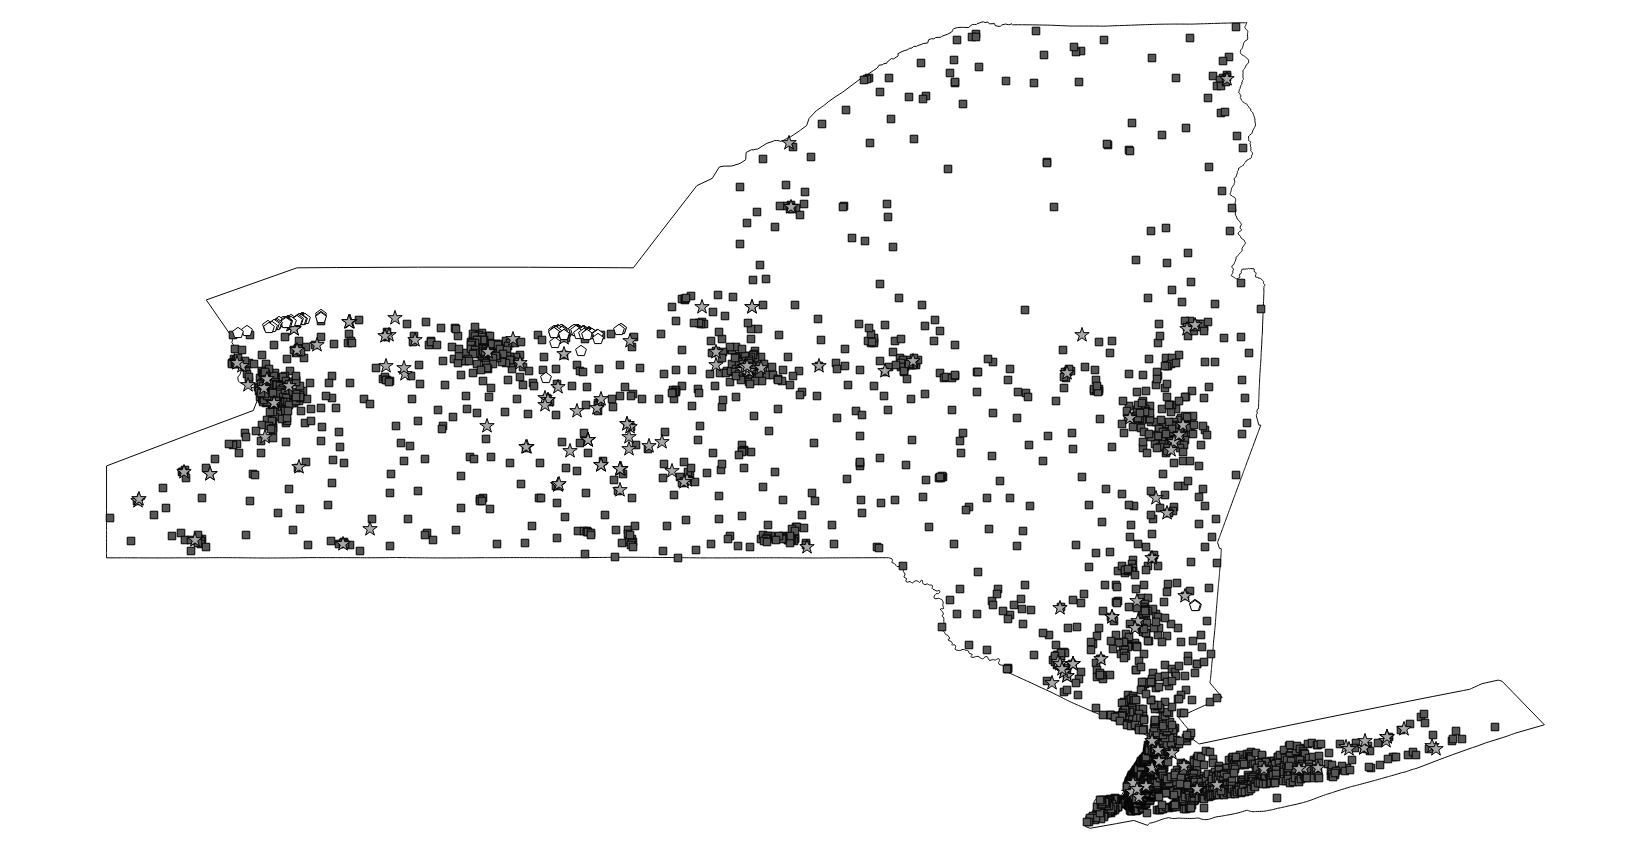
\includegraphics[scale=.4]{network_66}
\caption{This shows something}
\end{framed}
\end{figure}

\begin{figure}
\centering
\begin{framed}
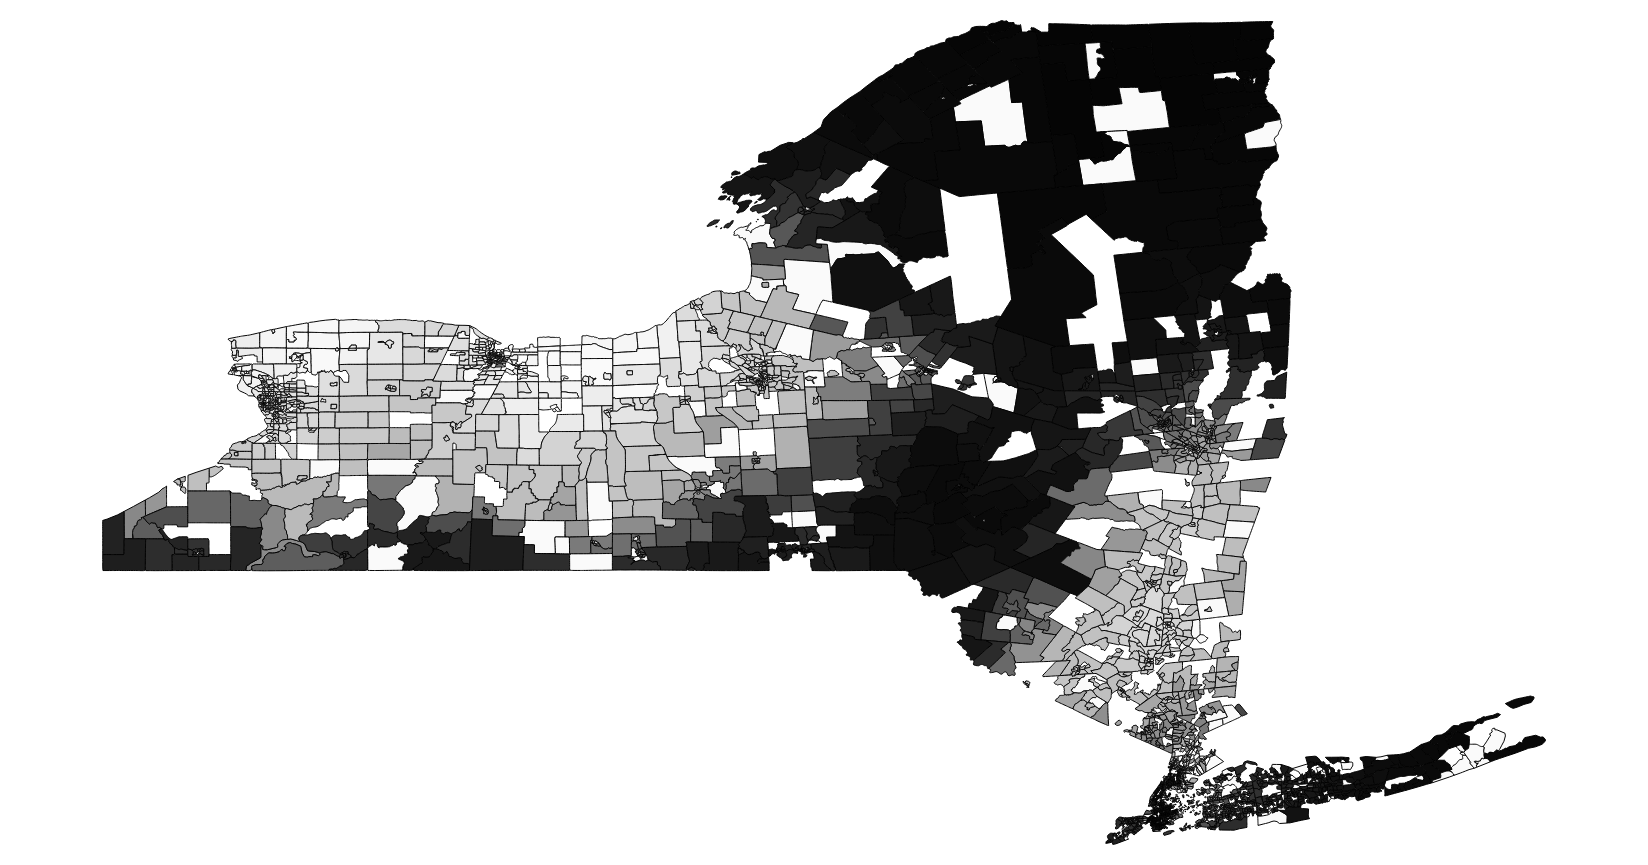
\includegraphics[scale=.4]{prices_66}
\caption{This shows something}
\end{framed}
\end{figure}

\subsection{Grape Farms}

\begin{table}
\centering
\begin{framed}
\begin{tabular}{c|c|c|c}%
	Type&Average&Variance&Deviation
    \csvreader[head to column names]{price_69.csv}{}% use head of csv as column names
    {\\\hline \csvcoli & \csvcolii & \csvcoliii & \csvcoliv}
\end{tabular}
\caption{Another table caption}
\end{framed}
\end{table}

\begin{table}
\centering
\begin{framed}
\begin{tabular}{c|c|c|c|c}%
	Type&Max Price&Max County&Min Price&Min County
    \csvreader[head to column names]{county_69.csv}{}% use head of csv as column names
    {\\\hline \csvcoli & \csvcolii & \csvcoliii & \csvcoliv & \csvcolv}
\end{tabular}
\caption{Another table caption}
\end{framed}
\end{table}

\begin{figure}
\centering
\begin{framed}
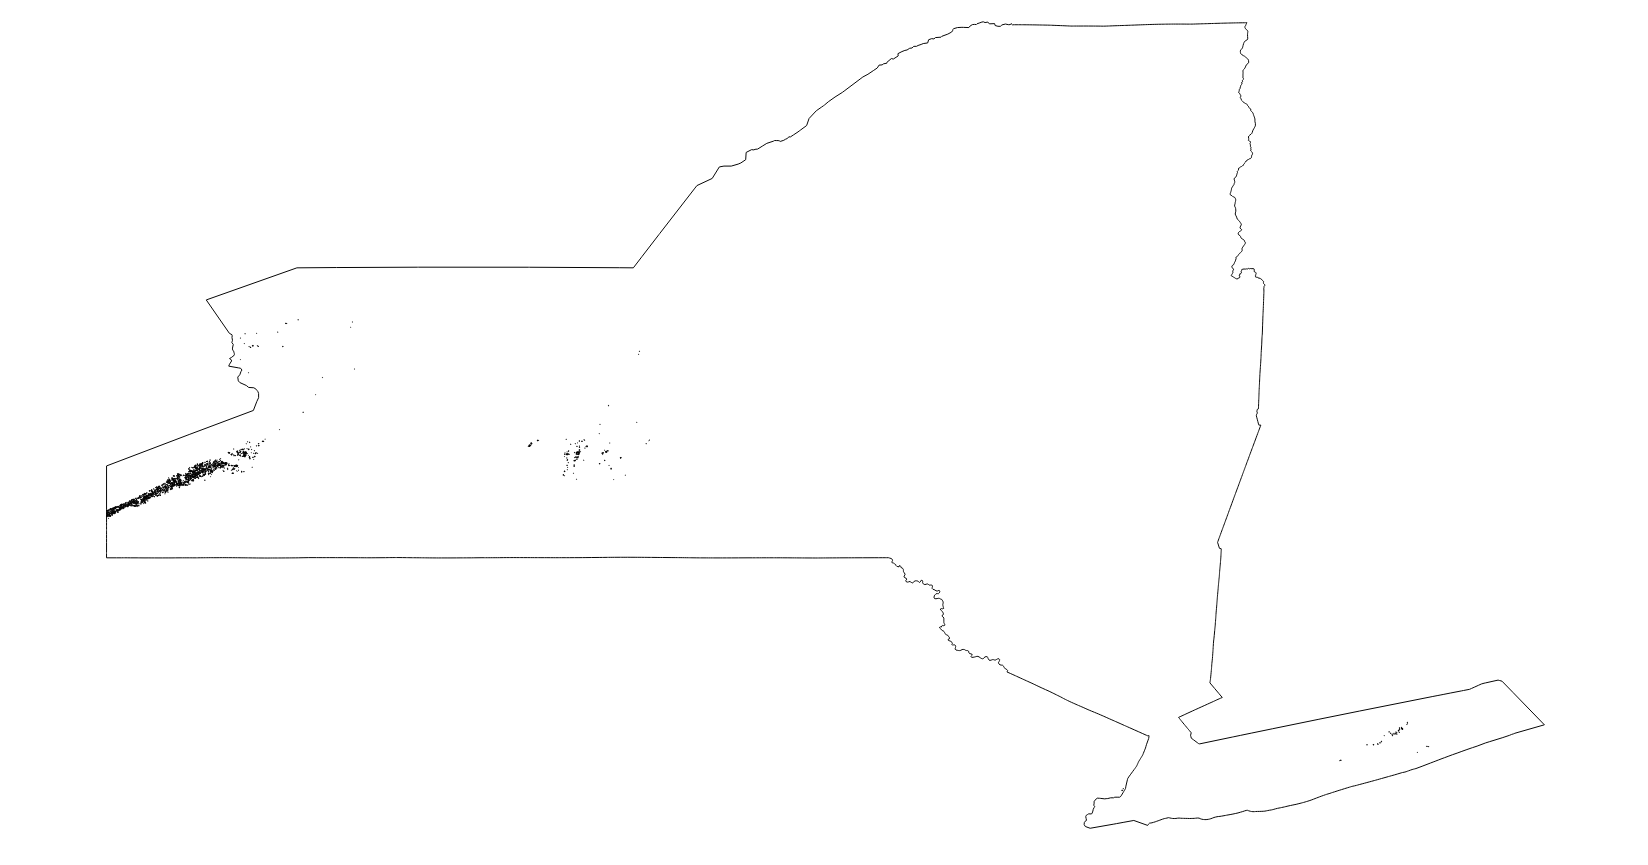
\includegraphics[scale=.4]{farms_69}
\caption{This shows something}
\label{fig:farms_69}
\end{framed}
\end{figure}

\begin{figure}
\centering
\begin{framed}
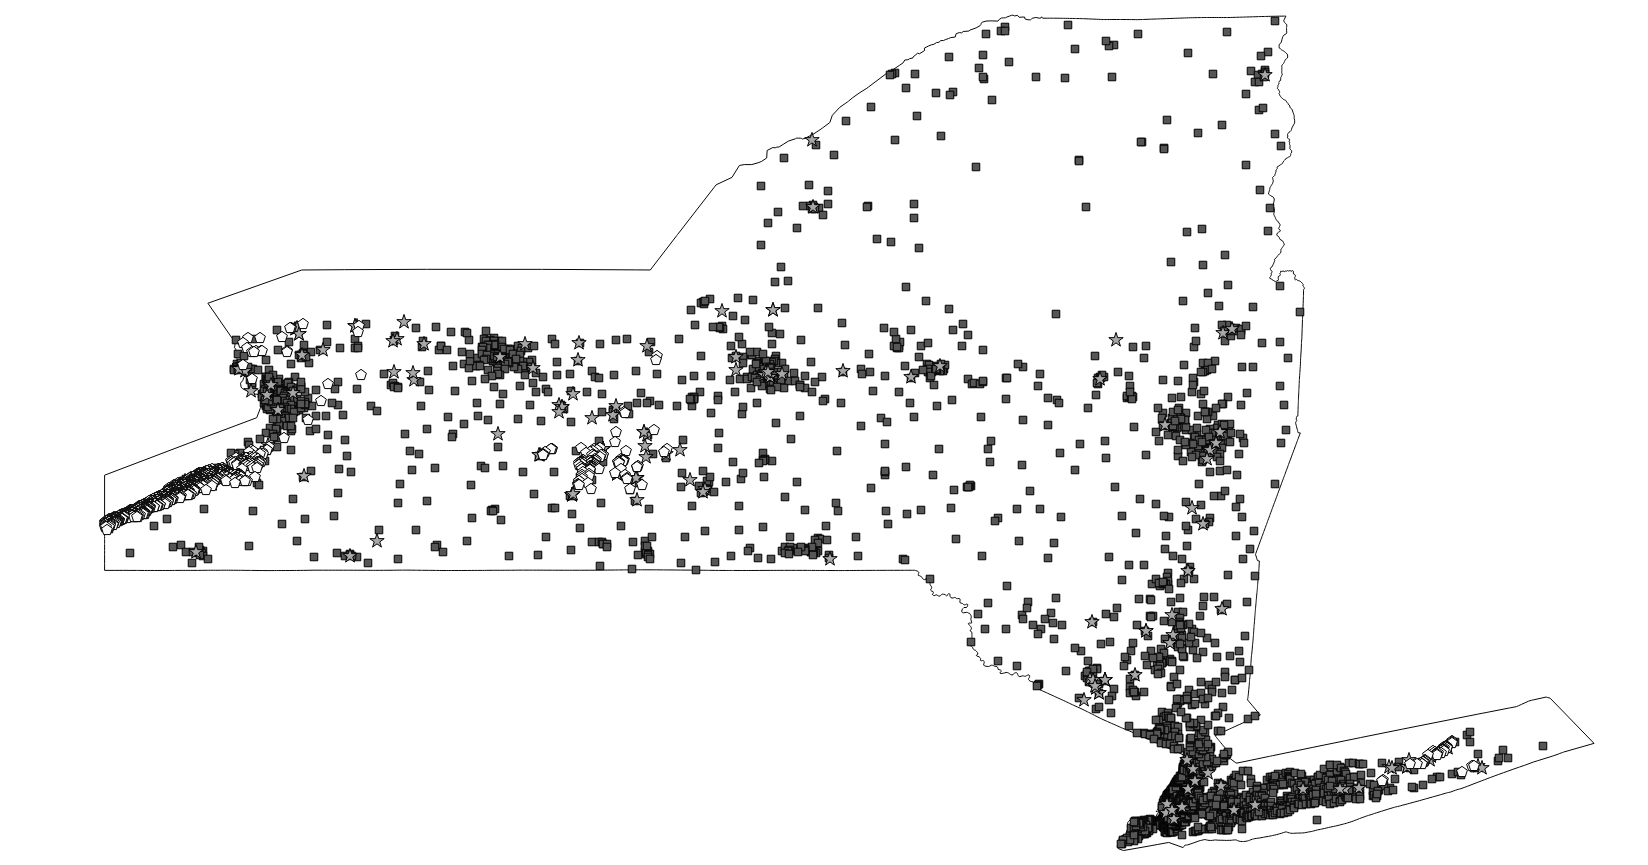
\includegraphics[scale=.4]{network_69}
\caption{This shows something}
\end{framed}
\end{figure}

\begin{figure}
\centering
\begin{framed}
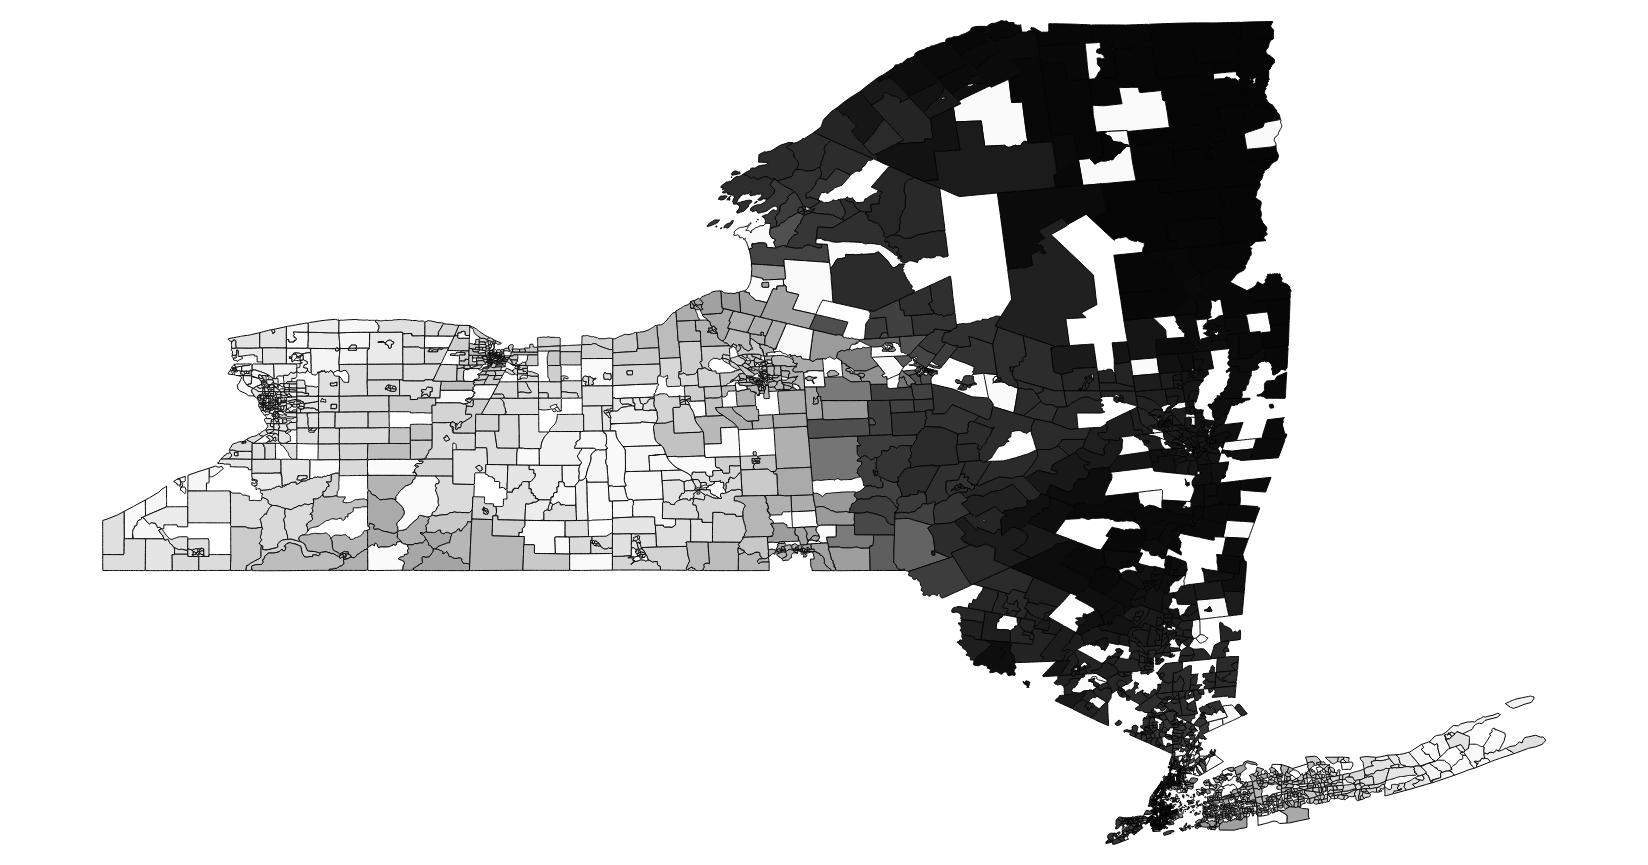
\includegraphics[scale=.4]{prices_69}
\caption{This shows something}
\end{framed}
\end{figure}

\subsection{Cabbage Farms}

Cabbages actually ended up being the most interesting band. The variance in the prices calculated by the algorithm is a lot lower as we can see in Table \ref{tab:price_243}. As you can see in Figure \ref{fig:farms_243} there are more individual cabbage farms. They are more spread apart and there is less variance in terms of their size.

\begin{table}
\centering
\begin{framed}
\begin{tabular}{c|c|c|c}%
	Type&Average&Variance&Deviation
    \csvreader[head to column names]{price_243.csv}{}% use head of csv as column names
    {\\\hline \csvcoli & \csvcolii & \csvcoliii & \csvcoliv}
\end{tabular}
\caption{Another table caption}
\label{tab:price_243}
\end{framed}
\end{table}

\begin{table}
\centering
\begin{framed}
\begin{tabular}{c|c|c|c|c}%
	Type&Max Price&Max County&Min Price&Min County
    \csvreader[head to column names]{county_243.csv}{}% use head of csv as column names
    {\\\hline \csvcoli & \csvcolii & \csvcoliii & \csvcoliv & \csvcolv}
\end{tabular}
\caption{Another table caption}
\end{framed}
\end{table}

\begin{figure}
\centering
\begin{framed}
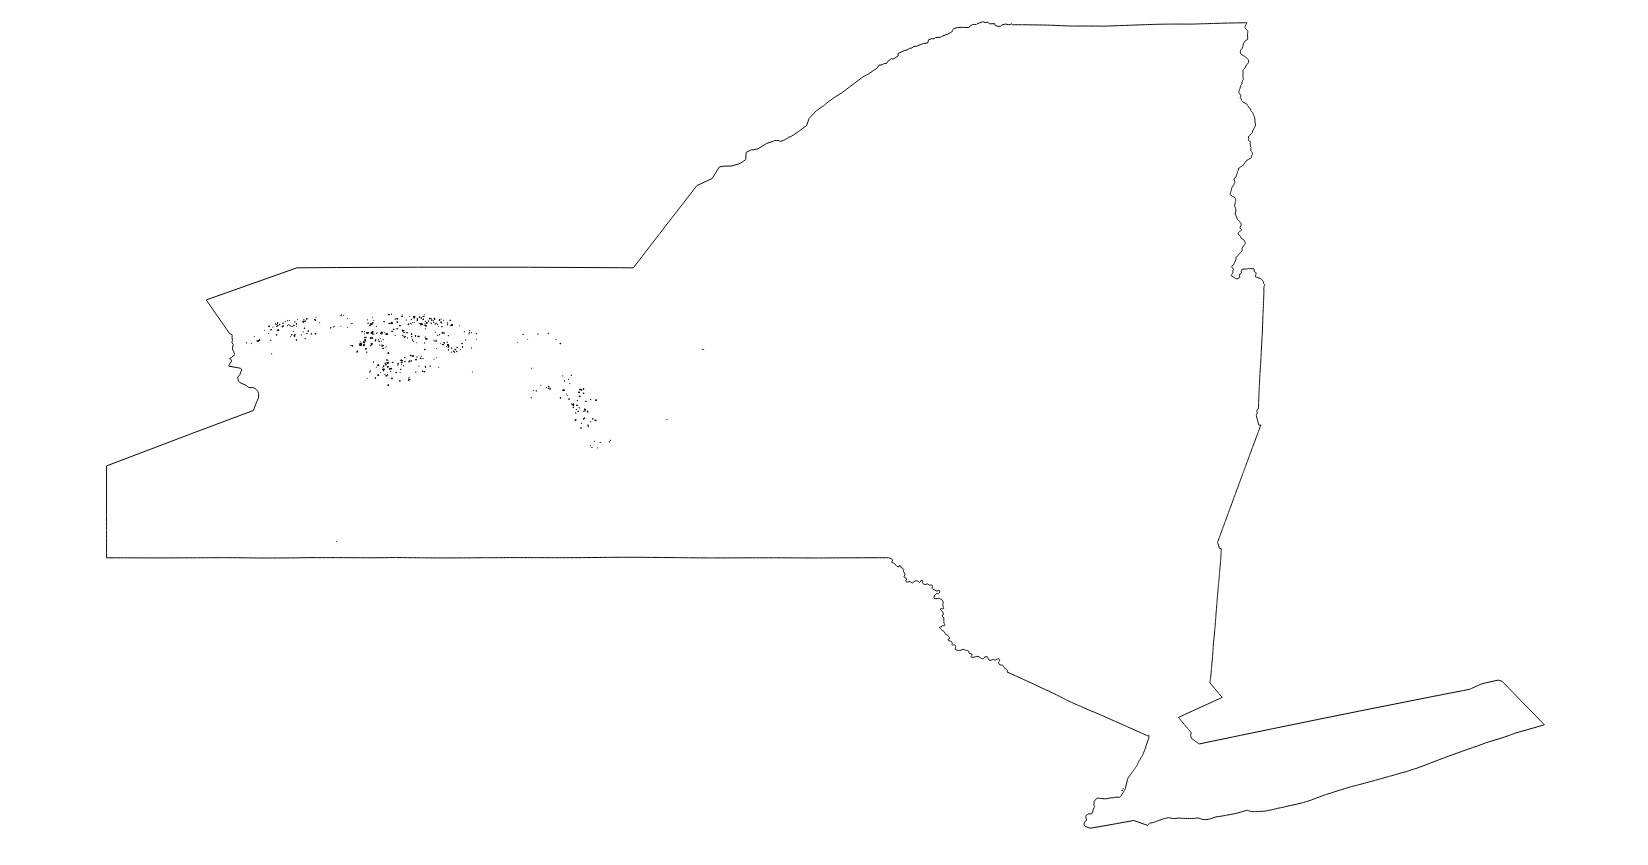
\includegraphics[scale=.4]{farms_243}
\label{fig:farms_243}
\caption{This shows something}
\end{framed}
\end{figure}

\begin{figure}
\centering
\begin{framed}
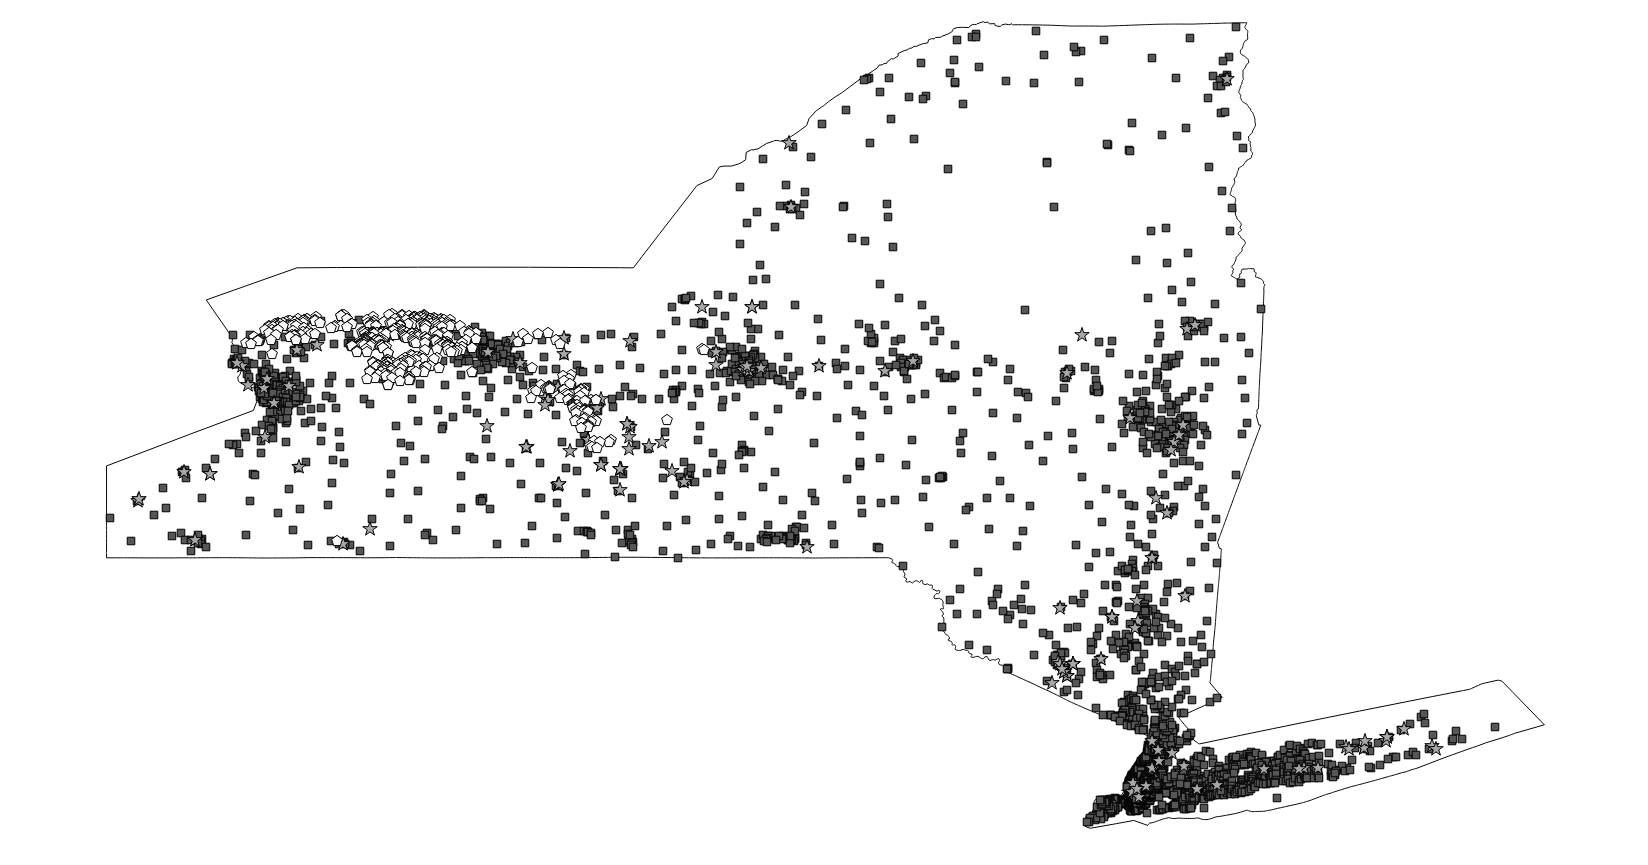
\includegraphics[scale=.4]{network_243}
\caption{This shows something}
\end{framed}
\end{figure}

\begin{figure}
\centering
\begin{framed}
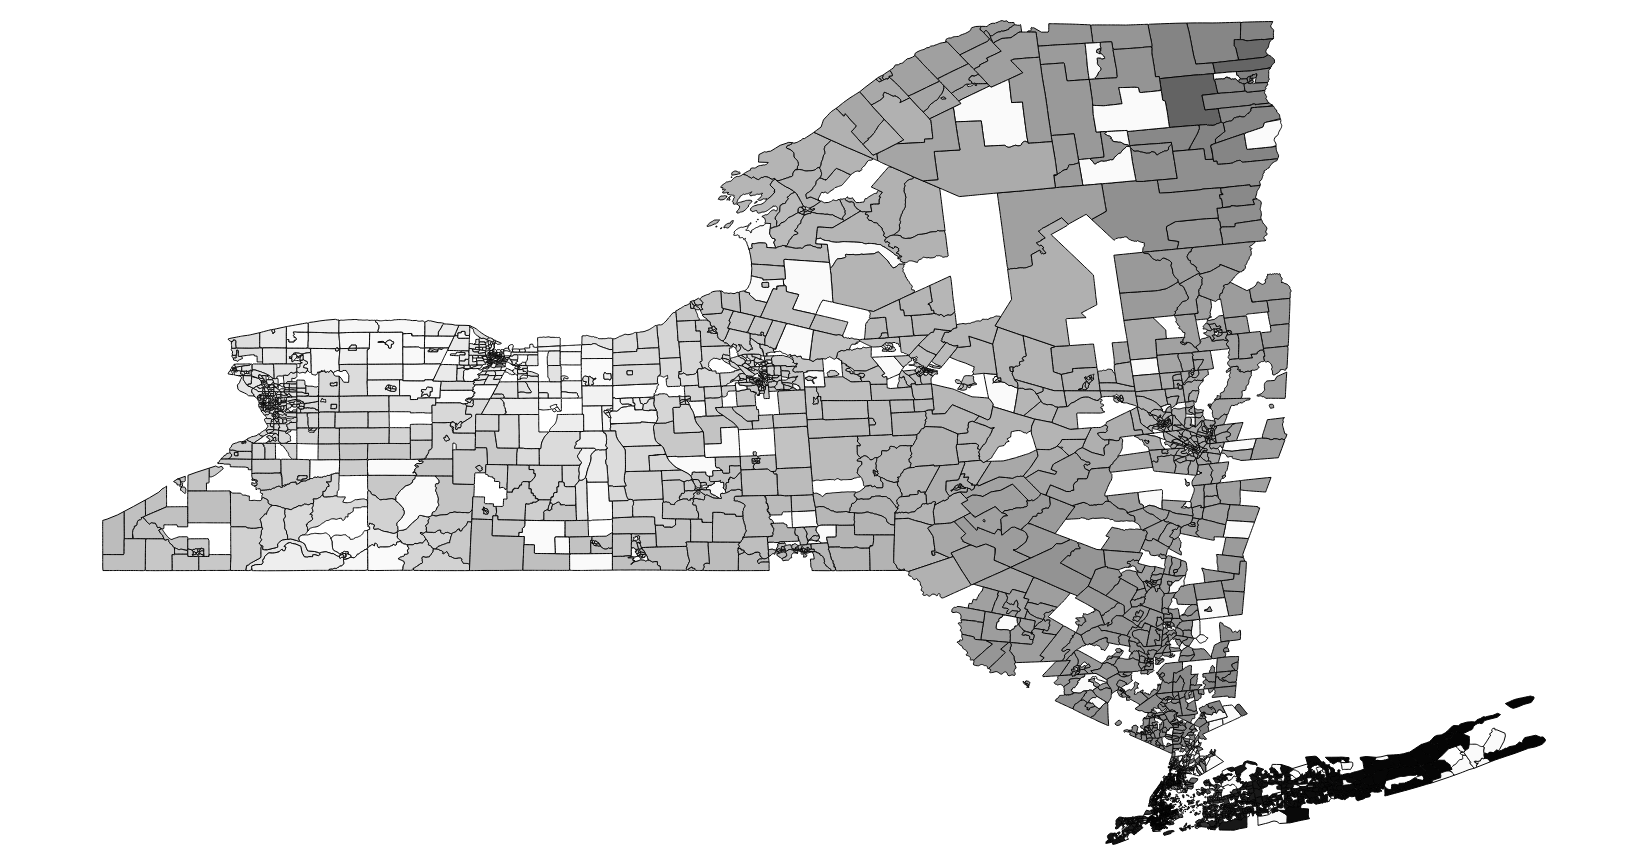
\includegraphics[scale=.4]{prices_243}
\caption{This shows something}
\end{framed}
\end{figure}

\section{Discussion}

\subsection{Comparing Different Results}

The differences in the solutions created by the different bands seemed to be explained mostly by the differences in the distribution of the farms throughout the state. This is most likely related to the fact that processors and stores stay pretty the much the same for each of the goods. Considering that store and for the most part intermediate processors stay constant between the various bands in the problem, it becomes obvious the aspect of the network that changed is the farms.

\subsubsection{Farms}

\begin{table}
\centering
\begin{framed}
\begin{tabular}{c|c|c|c}%
	Band&Average&Variance&Deviation
    \csvreader[head to column names]{farm_price.csv}{}% use head of csv as column names
    {\\\hline \csvcoli & \csvcolii & \csvcoliii & \csvcoliv}
\end{tabular}
\caption{Another table caption}
\end{framed}
\end{table}

\begin{table}
\centering
\begin{framed}
\begin{tabular}{c|c|c|c|c}%
	Band&Max Price&Max County&Min Price&Min County
    \csvreader[head to column names]{farm_county.csv}{}% use head of csv as column names
    {\\\hline \csvcoli & \csvcolii & \csvcoliii & \csvcoliv & \csvcolv}
\end{tabular}
\caption{Another table caption}
\end{framed}
\end{table}

\subsubsection{Intermediate Processors}

\begin{table}
\centering
\begin{framed}
\begin{tabular}{c|c|c|c}%
	Band&Average&Variance&Deviation
    \csvreader[head to column names]{proc_price.csv}{}% use head of csv as column names
    {\\\hline \csvcoli & \csvcolii & \csvcoliii & \csvcoliv}
\end{tabular}
\caption{Another table caption}
\end{framed}
\end{table}

\begin{table}
\centering
\begin{framed}
\begin{tabular}{c|c|c|c|c}%
	Band&Max Price&Max County&Min Price&Min County
    \csvreader[head to column names]{proc_county.csv}{}% use head of csv as column names
    {\\\hline \csvcoli & \csvcolii & \csvcoliii & \csvcoliv & \csvcolv}
\end{tabular}
\caption{Another table caption}
\end{framed}
\end{table}


\begin{figure}
\centering
\begin{framed}
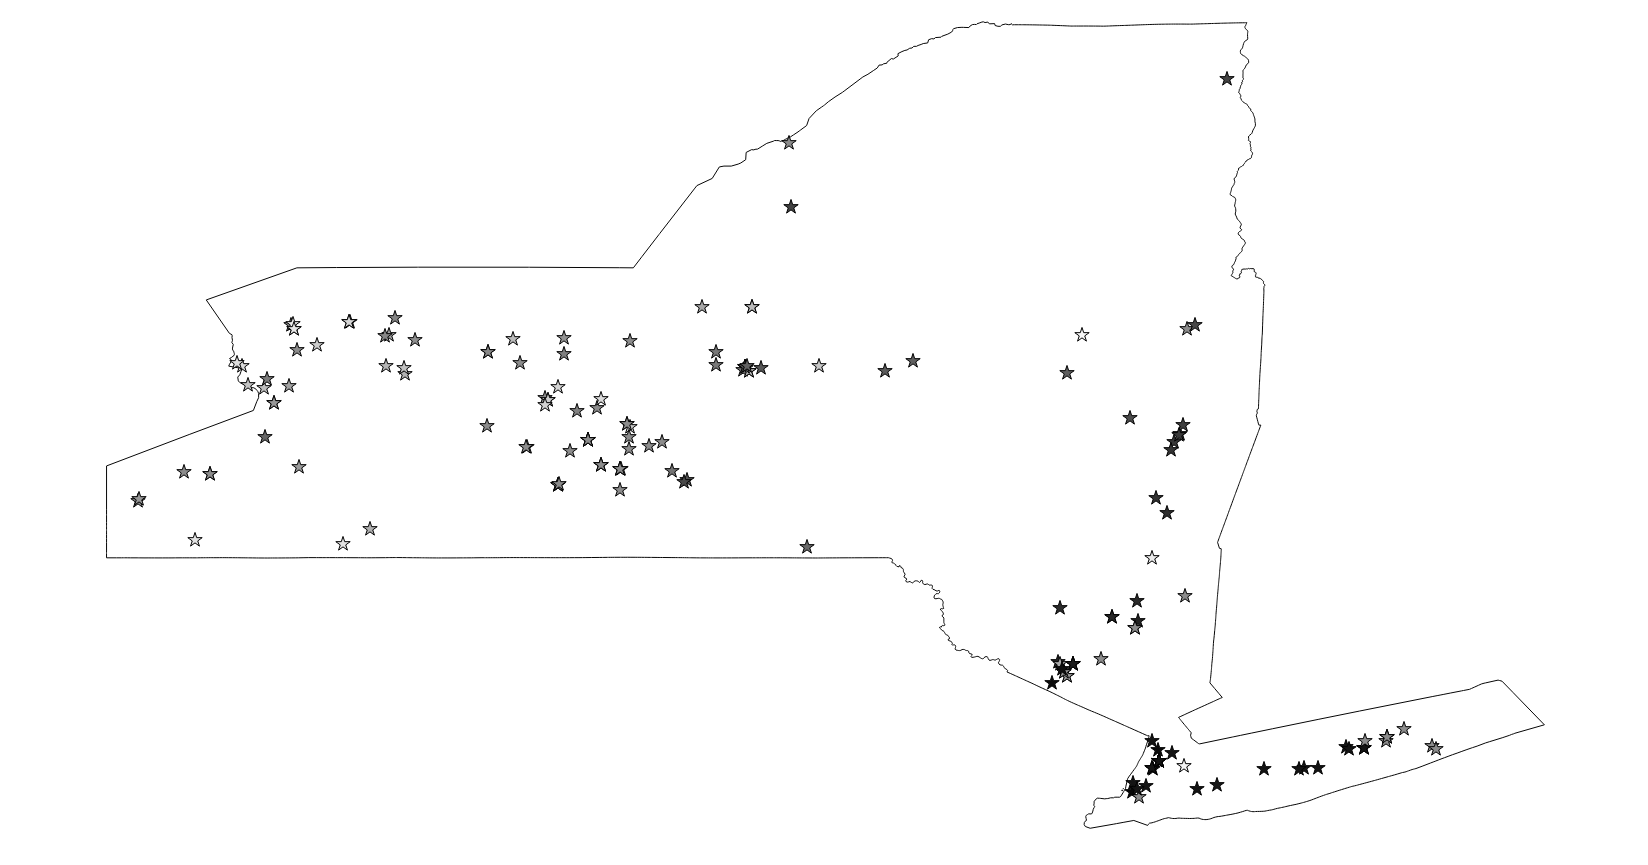
\includegraphics[scale=.4]{procs_243_49}
\caption{This shows something}
\end{framed}
\end{figure}

\begin{figure}
\centering
\begin{framed}
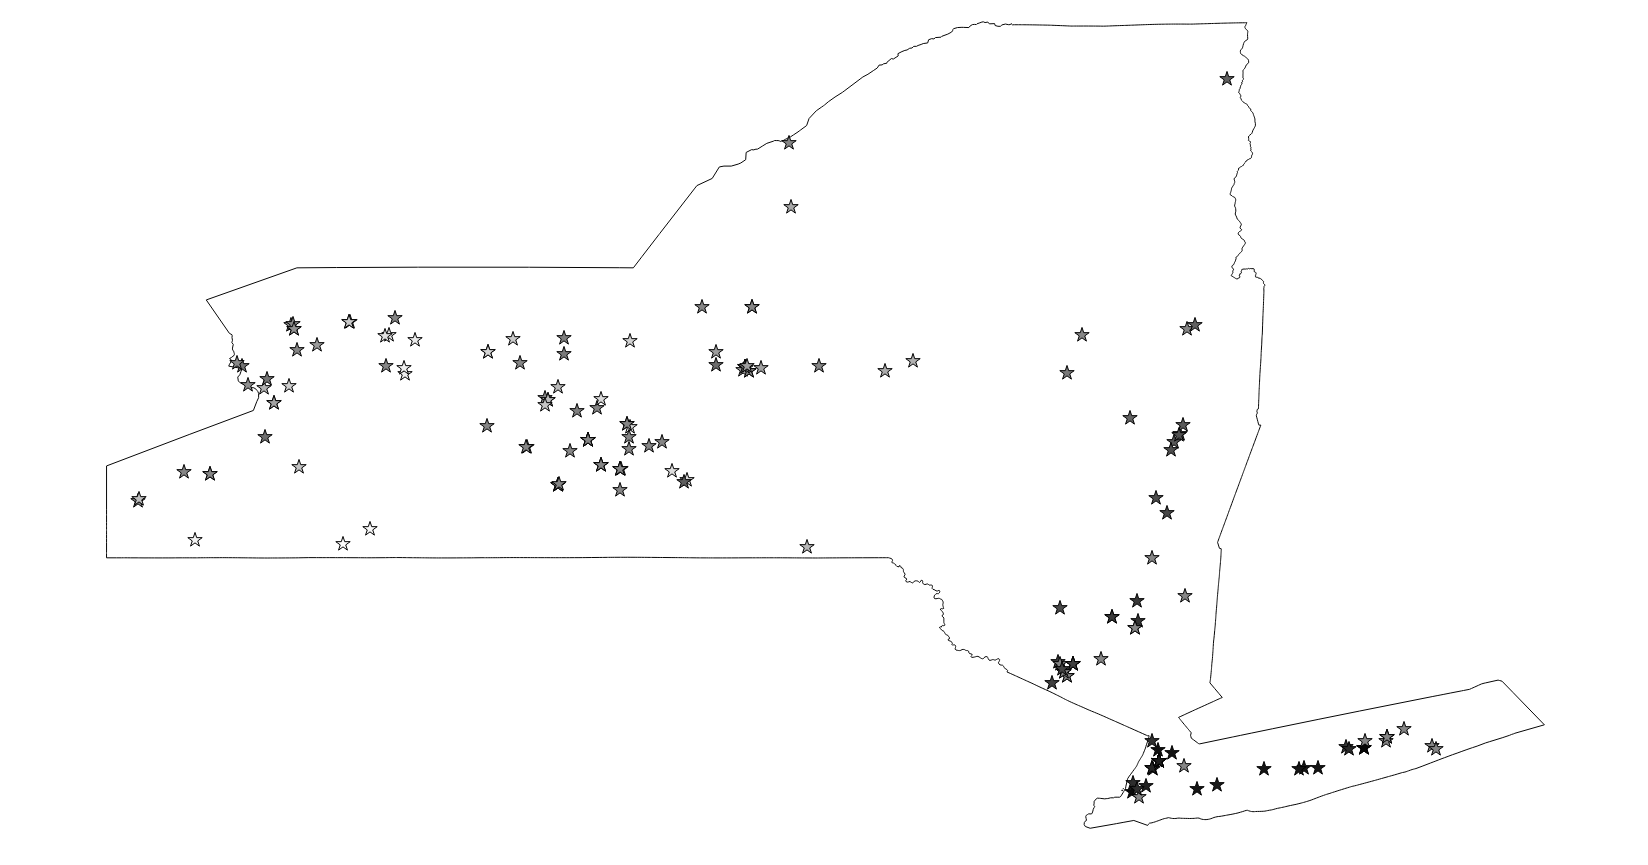
\includegraphics[scale=.4]{procs_243_66}
\caption{This shows something}
\end{framed}
\end{figure}

\begin{figure}
\centering
\begin{framed}
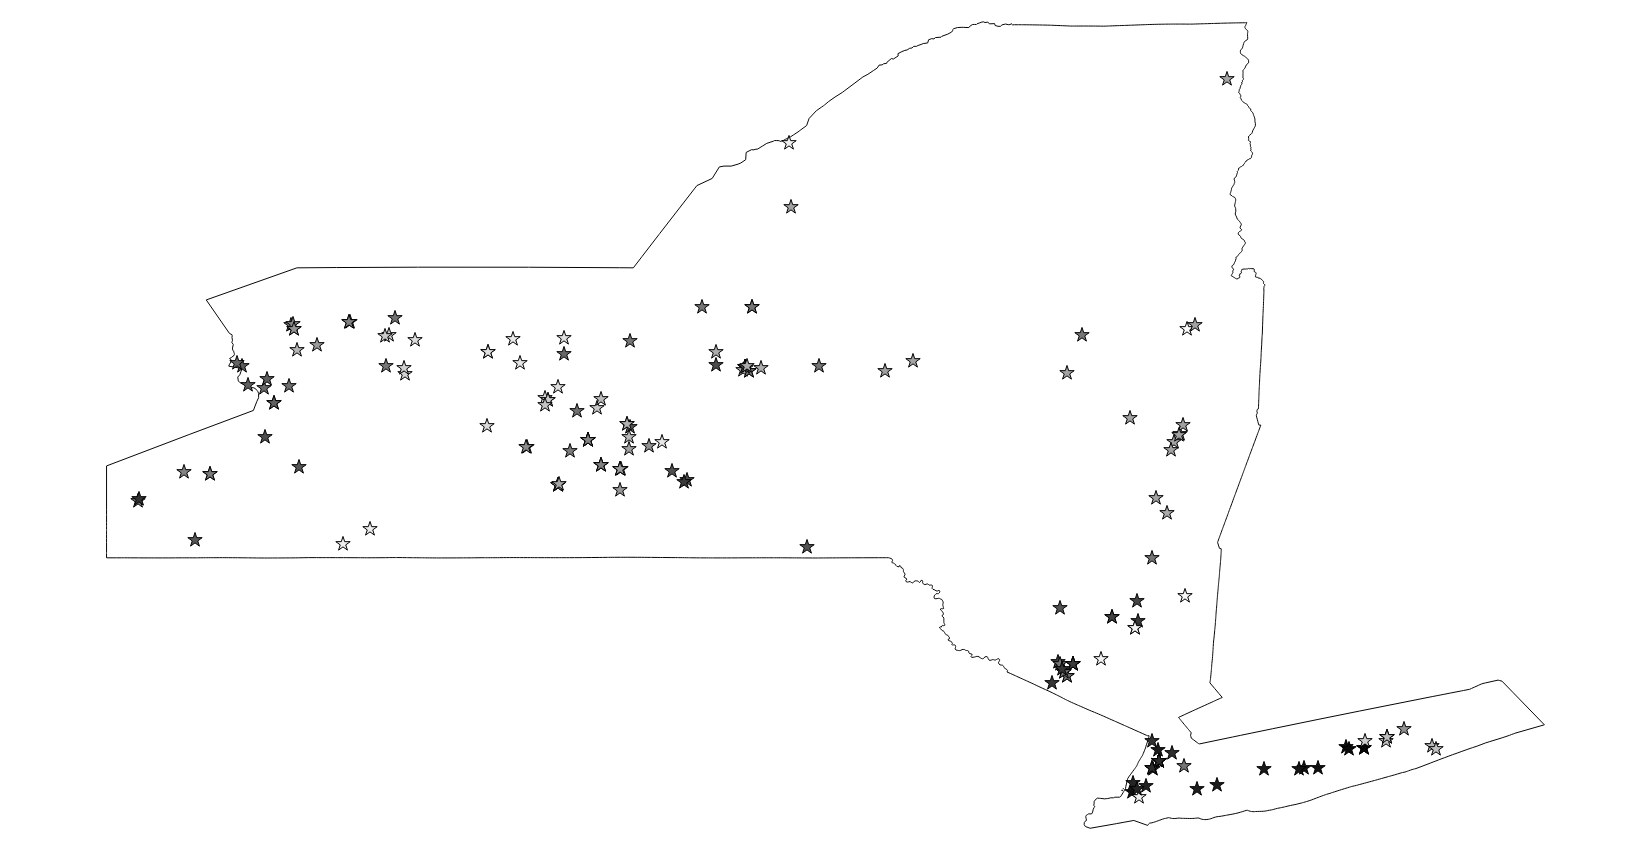
\includegraphics[scale=.4]{procs_243_69}
\caption{This shows something}
\end{framed}
\end{figure}

\subsubsection{Stores}

\begin{figure}
\centering
\begin{framed}
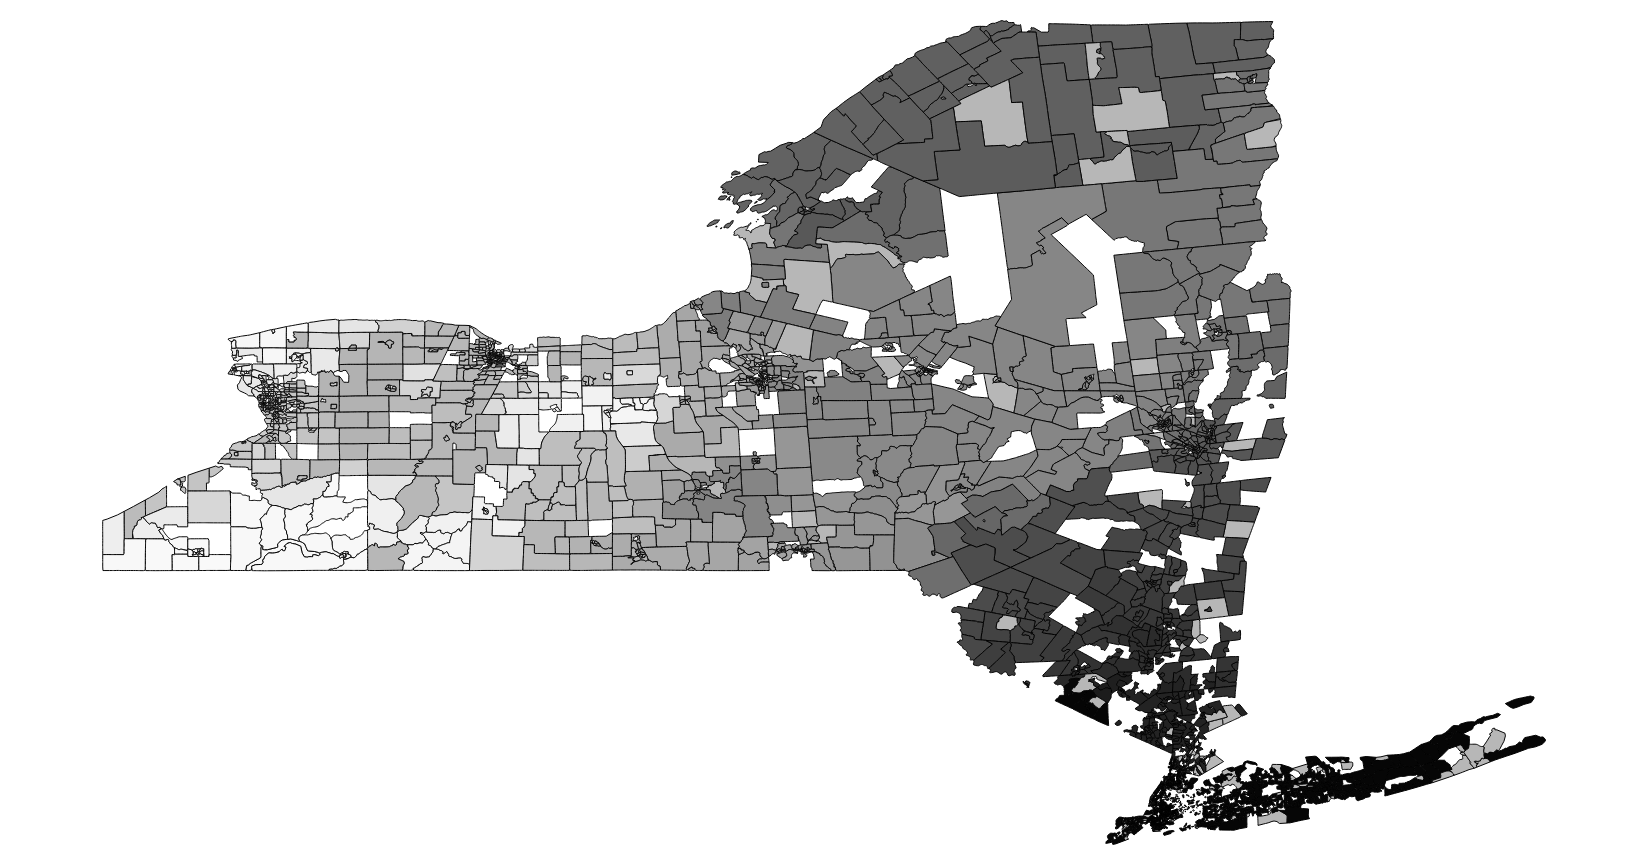
\includegraphics[scale=.4]{stores_243_49}
\caption{This shows something}
\end{framed}
\end{figure}

\begin{figure}
\centering
\begin{framed}
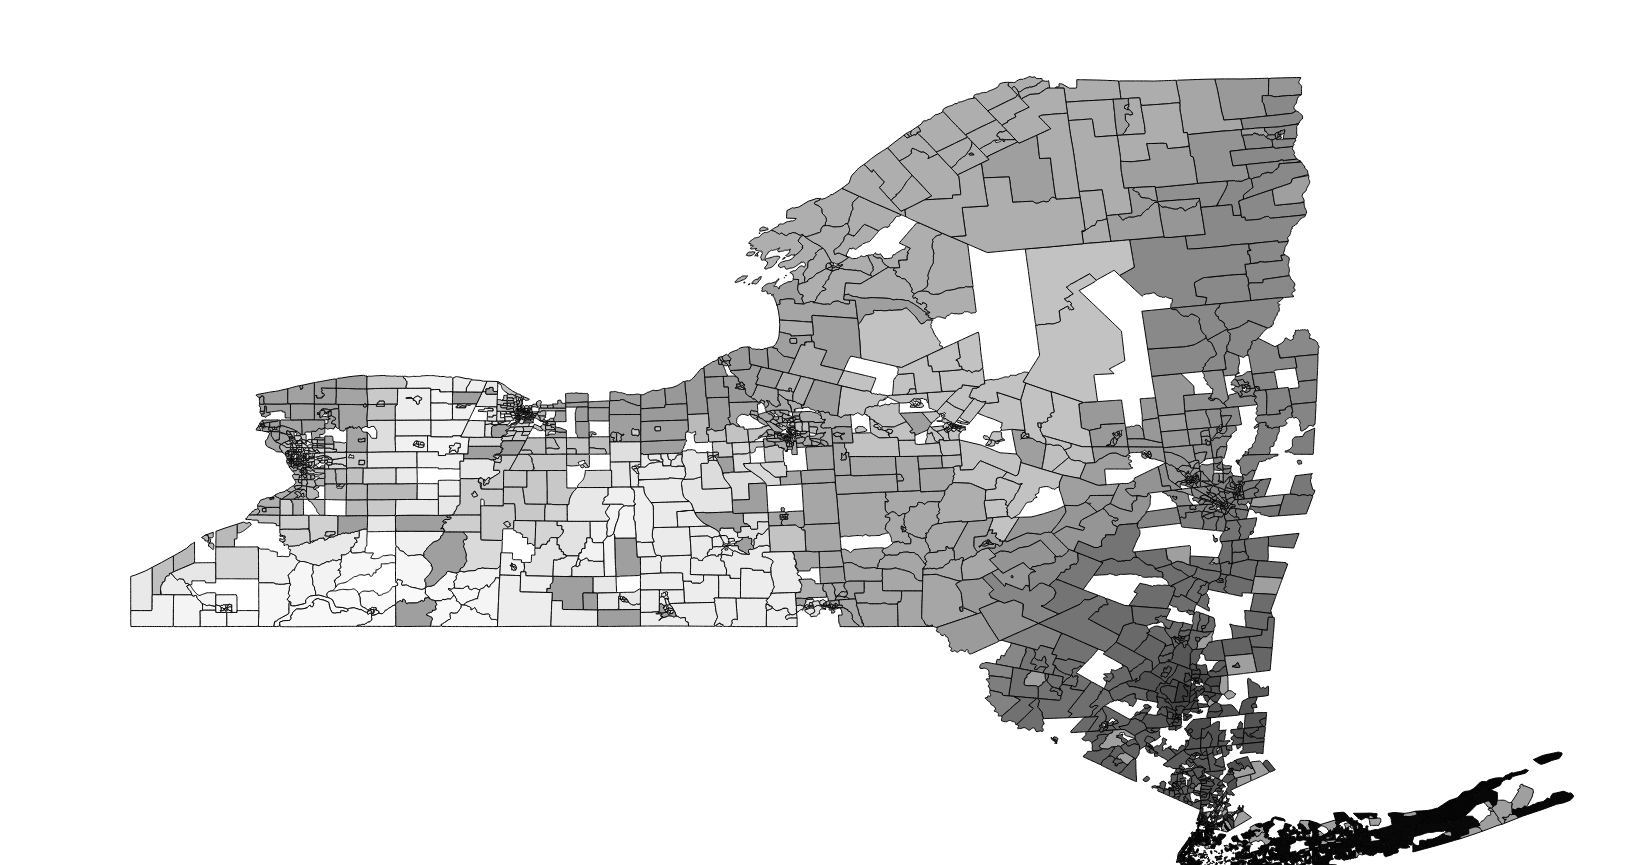
\includegraphics[scale=.4]{stores_243_66}
\caption{This shows something}
\end{framed}
\end{figure}

\begin{figure}
\centering
\begin{framed}
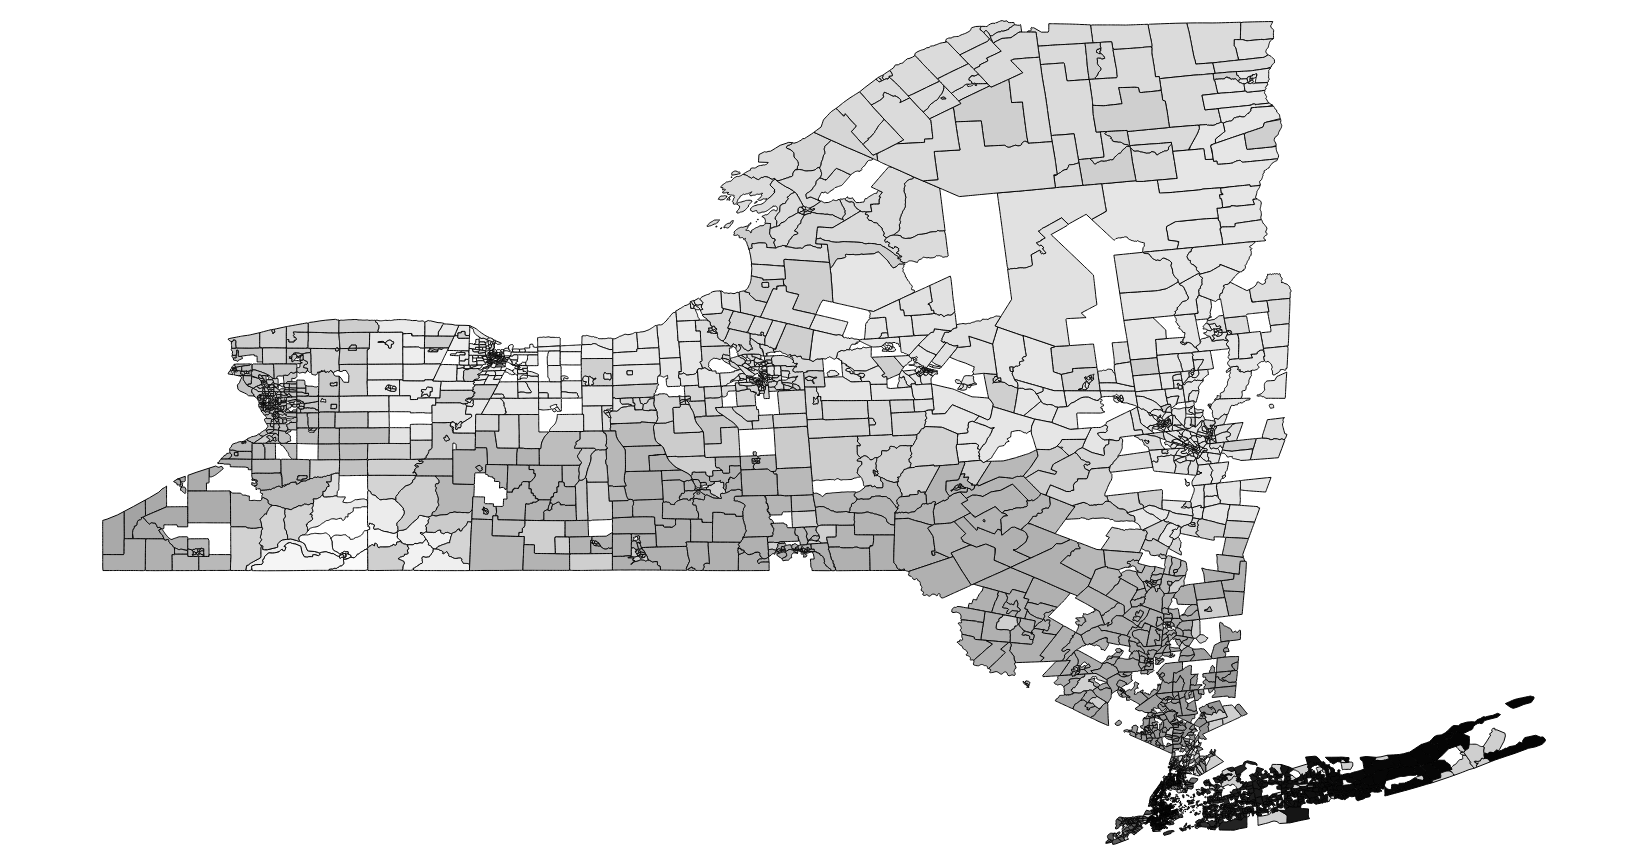
\includegraphics[scale=.4]{stores_243_69}
\caption{This shows something}
\end{framed}
\end{figure}

\begin{table}
\centering
\begin{framed}
\begin{tabular}{c|c|c|c}%
	Band&Average&Variance&Deviation
    \csvreader[head to column names]{store_price.csv}{}% use head of csv as column names
    {\\\hline \csvcoli & \csvcolii & \csvcoliii & \csvcoliv}
\end{tabular}
\caption{Another table caption}
\end{framed}
\end{table}


\begin{table}
\centering
\begin{framed}
\begin{tabular}{c|c|c|c|c}%
	Band&Max Price&Max County&Min Price&Min County
    \csvreader[head to column names]{store_county.csv}{}% use head of csv as column names
    {\\\hline \csvcoli & \csvcolii & \csvcoliii & \csvcoliv & \csvcolv}
\end{tabular}
\caption{Another table caption}
\end{framed}
\end{table}



\subsection{Robustness of Solutions}

For each of the bands, I tried to find an alternate solutions to the linear program in four ways using complementary slackness. Essentially, I parsed the value of the objective function from the solution file and added it as a constraint. Then I added constraints that tried pushing the maximum price to be higher or lower than it was in the original solution. I also tried pushing the minimum price to be lower or higher than it was in the solution.
I was able to change get a second solution accross all bands, but the differences weren't drastic. In each file at most roughly 500 prices of the roughly 8000 prices across farms and stores changed. Most importantly the minimum and maximum values didn't change by more than 10 percent. I can provide the other difference tables with this data as a .csv files upon request if you want to look through them in detail. They can also be generated using the git repository. They are rather cumbersome (there are 16 of them, each with between 50 and 500 lines), and I couldn't figure out how to elegantly display them.
To be honest, I think the changes have more to do with rounding errors related to the way that python stores floating point numbers rather than actual differences to the solution. When the value of the objective function is parsed from the solution file into a python float the last decimal point may not be accurate. In fact, in all cases the objective function was not exactly accurate.

\subsection{Transportation Problem Assumptions}

Despite the possibilities, prices in a transportation problem aren't a perfect analogue to market prices. Transportation problems assume firms coordinate to reduce total transportation costs. Additionally, prices in the problem only reflect linear transportation costs. To make the problem more realistic, we can increase all prices by a constant amount to reflect inputs (assuming constant returns to scale). Under this change, the solution is still optimal from a social planning perspective. 

Additionally, I am looking into better specifying the transportation problem using the Google Maps and MapQuest API.  My specification makes assumptions about connections between farms, factories, and retailers that may not exist for contractual reasons. In reality, fresh produce can be altered or stored at intermediaries, there may be capacities on the intermediate nodes, and intermediate nodes that buy less than 10,000 dollars of produce. 

Finally, I under-estimate costs because New York exports fresh produce. Adding demand from out-of-state increases costs in-state.  That being said, the estimated prices are still economically significant without exports. They represent a minimum for prices; adding additional demand from out-of-state increases costs in-state. Additionally, most of the categories of produce have a short shelf life and are exported in insignificant quantities with the exception of apples.


\subsection{Comparing Optimal Transport with OLS}

One key question is how I've skipped doing exclusion restrictions and the such to do my model. The other question is how I've come up with point estimates when most empirical models come up with ranges. The final thing is it might be foolish to look at the data in this way. I've probably lost a lot by ignoring the traditional techniques economist use make estimates about supply and demand. That being said, I think there is something here. There is a ton of potential in refining this technique more and more so that it's as polished as the techniques involved with ordinary least squares


\subsection{Conclusion}
Instead of just jumping into my project. I figured I wanted to take a moment to reflect and explain why I've done what I've done. I've brought together a lot of cool tools from mapping and geographic imaging, optimization, and of course economics. I've tried my best to fit these tools together in a way that makes sense, but that's one of the hard things about looking about using a well established tool in an unconventional way. In some ways, it may not make sense. Either way, I definitely want to say it's been a fun and exciting process to see the resources that are out there beyond FRED, the BLS, and NCYS and would highly recommend to others to check it out and not be afraid when the file extension isn't .csv.

The second thing is Food is super complicated, I've created a model where I tried to capture the elements of the food transportation system that I thought were important. Obviously, there is room for improvement in terms of specifying the problem especially with reguards to the sellers.

\pagebreak

\begin{thebibliography}{99}
\bibitem{Bernell}Bernell, S., Weber, B., {\&} Edwards, M. (2006). Restricted Opportunities, Personal Choices, Ineffective Policies: What Explains Food Insecurity in Oregon? Journal of Agricultural and Resource Economics, 31(2), 193-211. 
\bibitem{Chung} Chung, Chanjin, and Samuel L. Myers. "Do the Poor Pay More for Food? An Analysis of Grocery Store Availability and Food Price Disparities." The Journal of Consumer Affairs 33.2 (1999): 276-96.
\bibitem{Cook} Cook, W. J., Cunningham, W. H., Pulleyblank, W. R.,  {\&}  Schrijver, A. (1998). Combinatorial optimization (pp. 91-126). New York: John Wiley  {\&}  Sons.
\bibitem{Hwang} Hwang, M., {\&} Smith, M. (2012). Integrating publicly available web mapping tools for cartographic visualization of community food insecurity: A prototype. GeoJournal, 77(1), 47-62.
\bibitem{Just} Just, R., {\&} Weninger, Q. (1997). Economic Evaluation of the Farmers' Market Nutrition Program. American Journal of Agricultural Economics, 79(3), 902-917.
\bibitem{dfs} NYS Division of Food Safety {\&} Inspection (2016). Retail Food Stores [Download table]. Retrieved from \url{https://data.ny.gov/Economic-Development/Retail-Food-Stores/9a8c-vfzj}
\bibitem{dam} NYS Department of Agriculture and Markets (DAM) (2016). Farm Product Dealer Licenses Currently Issued [Download table]. Retrieved from \url{https://data.ny.gov/Economic-Development/Retail-Food-Stores/9a8c-vfzj}
\bibitem{Larson} Larson, J., {\&} Moseley, W. (2012). Reaching the limits: A geographic approach for understanding food insecurity and household hunger mitigation strategies in Minneapolis-Saint Paul, USA. GeoJournal, 77(1), 1-12.
\bibitem{Stewart} Stewart, T., {\&} Ittmann, H. (1979). Two-Stage Optimization in a Transportation Problem. The Journal of the Operational Research Society, 30(10), 897-904.
\bibitem{census} U.S. Census Bureau. (2011). American Community Survey, 2010 ACS 5-year Selected Population Tables [Table B25077]. Retrieved from \url{https://factfinder.census.gov/faces/nav/jsf/pages/download_center.xhtml}
\bibitem{nass} USDA, NASS. (2011). USDA, National Agricultural Statistics Service, 2010 New York Cropland Data Layer [Download]. Retrieved from \url{http://cugir.mannlib.cornell.edu/bucketinfo.jsp?id=8033}

\end{thebibliography}



\end{document}